\باب{ کارناف نقشہ جات} 
بوولین جدول سے کسی بھی تفاعل کی مساوات بذریعہ مجموعہ ارکان ضرب یا  ضرب بعد از جمع حاصل کر کے اسے گیٹوں کی مدد سے جامہ پہنایا جا سکتا ہے۔عموماً، اس مساوات میں گیٹوں کی تعداد اور فی گیٹ مداخل کی تعداد کم کی جا سکتی ہے۔ کم مداخل کے، کم تعداد گیٹ استعمال کرنے سے عددی دور پر کم لاگت آئے گی۔ تفاعل کی سادہ صورت بوولین منطق سے حاصل کی جا سکتی ہے، البتہ ایک نہایت عمدہ اور سادہ طریقہ کار جسے کارناف نقشہ جات کی ترکیب کہتے ہیں، استعمال کیا جاتا ہے۔اس باب میں اس ترکیب پر غور کیا جائے گا۔یہ ترکیب چار اور چار سے کم آزاد متغیرات کے تفاعل کی سادہ صورت حاصل کرنے میں نہایت آسان ثابت ہو گا۔

\حصہ{کارناف نقشے کا بنیادی خاکہ}
دو آزاد متغیر تفاعل \عددی{F(x,y)} کے بوولین جدول میں چار مختلف ارکان ضرب ہوں گے، جنہیں جدول \حوالہ{جدول_کارناف_دو_آزاد} میں پیش کیا گیا ہے۔ اس کے \اصطلاح{ کارناف نقشے }\فرہنگ{کارناف نقشہ}\حاشیہب{Karnaugh map}\فرہنگ{Karnaugh map} میں چار خانے ہوں گے، جہاں ایک خانہ ایک رکن ضرب کو ظاہر کرتا ہے۔ کارناف نقشے میں ان چار خانوں کی ترتیب، شکل \حوالہ{شکل_کارناف_بنیادی_صورت}-الف میں دکھائی گئی ہے،جہاں بالائی صف میں \عددی{x=0} جبکہ نچلی صف میں \عددی{x=1} ہے؛ یہ قیمتیں صفوں کے بائیں طرف، خانوں سے باہر، لکھی گئی ہیں۔اسی طرح بائیں قطار میں \عددی{y=0}جبکہ دائیں قطار میں \عددی{y=1}ہے؛ یہ قیمتیں خانوں سے باہر، قطاروں کے اوپر جانب لکھی گئی ہیں ۔یوں بالائی صف اور دائیں قطار کے مشترکہ خانے میں \عددی{x=0} اور \عددی{y=1} ہے۔اس خانے کے آزاد متغیرات کی ثنائی قیمتوں کو اکٹھے \عددی{01} لکھیں۔ یہ خانہ رکن ضرب \عددی{\overline{x}y} کو ظاہر کرتا ہے، لہٰذا اس خانے میں \عددی{\overline{x}y} (شکل-الف) یا \عددی{m_1} (شکل-ب) لکھا جائے گا۔باقی خانوں میں اسی طرح اندراج کیے جاتے ہیں۔شکل \حوالہ{شکل_کارناف_چار_متغیر_بنیادی_صورت} میں اسی طرز پر چار آزاد متغیر تفاعل کارناف نقشے میں خانہ \عددی{m_{11}} کی نشاندہی کی گئی ہے۔

 \begin{table}
 \caption{دو متغیر ارکان ضرب۔}
 \label{جدول_کارناف_دو_آزاد}
 \centering
\begin{otherlanguage}{english}
\begin{tabular}{CC|CC}
\toprule
x&y&&\\
\midrule
0&0&\overline{x}\,\overline{y}&m_0\\
0&1&\overline{x}y&m_1\\
1&0&x\overline{y}&m_2\\
1&1&xy&m_3\\
\bottomrule
\end{tabular}
\end{otherlanguage}
\end{table}
%
\begin{figure}
\centering
\begin{subfigure}{0.6\textwidth}
\centering
\begin{tikzpicture}
\pgfmathsetmacro{\kxstep}{1}
\pgfmathsetmacro{\kystep}{1}
\pgfmathsetmacro{\kpin}{0.75}
\draw[xstep=\kxstep,ystep=\kystep](0,0) grid (2*\kxstep,-2*\kystep);
\draw(0,0)--++(135:\kpin)node[pos=0.75,above right]{$y$}node[pos=0.75,below left]{$x$};
\draw(\kxstep/2,0)node[above]{$0$} ++(\kxstep,0)node[above]{$1$};
\draw(0,-\kystep/2)node[left]{$0$} ++(0,-\kystep)node[left]{$1$};
\draw(\kxstep/2,-\kystep/2)node[]{$\overline{x}\,\overline{y}$} ++(\kxstep,0)node[]{$\overline{x}y$};
\draw(\kxstep/2,-\kystep-\kystep/2)node[]{$x\overline{y}$} ++(\kxstep,0)node[]{$xy$};
\draw[gray](\kxstep,-\kystep/2) circle (1.1cm and 0.4cm);
\draw[](2*\kxstep+0.2,-\kystep/2) to [out=35,in=180]++(0.5,0.2)node[right]{\text{\RL{اس صف میں \عددی{x=0} ہے}}};
\draw[gray](1.5*\kxstep,-\kystep) circle (0.4cm and 1.05cm);
\draw[](1.5*\kxstep,-2*\kystep-0.05) to [out=-35,in=180]++(0.5,-0.2)node[right]{\text{\RL{اس قطار میں \عددی{y=1} ہے}}};
\end{tikzpicture}
\caption{}
\end{subfigure}\hfill
\begin{subfigure}{0.4\textwidth}
\centering
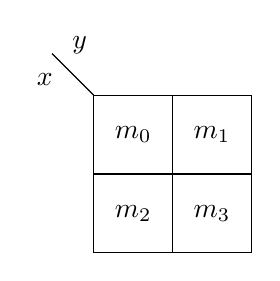
\begin{tikzpicture}
\pgfmathsetmacro{\kxstep}{1}
\pgfmathsetmacro{\kystep}{1}
\pgfmathsetmacro{\kpin}{0.75}
\draw[xstep=\kxstep,ystep=\kystep](0,0) grid (2*\kxstep,-2*\kystep);
\draw(0,0)--++(135:\kpin)node[pos=0.75,above right]{$y$}node[pos=0.75,below left]{$x$};
\draw(\kxstep/2,-\kystep/2)node[]{$m_0$} ++(\kxstep,0)node[]{$m_1$};
\draw(\kxstep/2,-\kystep-\kystep/2)node[]{$m_2$} ++(\kxstep,0)node[]{$m_3$};
\end{tikzpicture}
\caption{}
\end{subfigure}
\caption{دو آزاد متغیر کارناف نقشے کی بنیادی صورت۔}
\label{شکل_کارناف_بنیادی_صورت}
\end{figure}

تین آزاد متغیر تفاعل \عددی{F(x,y,z)} کے آٹھ ارکان ضرب ہوں گے۔ انہیں شکل \حوالہ{شکل_کارناف_تین_متغیر_بنیادی_صورت} کے \قول{\,  کارناف نقشہ }میں دکھایا گیا ہے۔اس شکل میں دو صف اور چار قطار ہیں۔صفوں کا تعین \عددی{x}کی قیمت، جبکہ قطاروں کا تعین \عددی{yz}کی قیمت کرتی ہے۔ان قیمتوں کو (ثنائی گنتی کے روپ میں نہیں بلکہ)گرے رمز میں لکھا جاتا ہے۔ یوں، بائیں ہاتھ سے شروع کر کے، پہلی قطار میں \عددی{yz} کی قیمت \عددی{00}، دوسری میں \عددی{01}،تیسری میں \عددی{11} جبکہ آخری قطار میں \عددی{10} ہو گی۔

\begin{figure}
\centering
\begin{tikzpicture}
\pgfmathsetmacro{\kxstep}{1}
\pgfmathsetmacro{\kystep}{1}
\pgfmathsetmacro{\kpin}{0.75}
\draw[xstep=\kxstep,ystep=\kystep](0,0) grid (4*\kxstep,-2*\kystep);
\draw(0,0)--++(135:\kpin)node[pos=0.75,above right]{$yz$}node[pos=0.75,below left]{$x$};
\foreach \kx/\xlb in {0/{00},1/{01},2/{11},3/{10}}{\draw(\kx*\kxstep+\kxstep/2,0)node[above]{$\xlb$};}
\foreach \ky/\ylb in {0/0,1/1}{\draw(0,-\ky*\kystep-\kystep/2)node[left]{$\ylb$};}
\foreach \kx/\xlb in {0/{m_0},1/{m_1},2/{m_3},3/{m_2}}{\draw(\kx*\kxstep+\kxstep/2,-\kystep/2)node[]{$\xlb$};}
\foreach \kx/\xlb in {0/{m_4},1/{m_5},2/{m_7},3/{m_6}}{\draw(\kx*\kxstep+\kxstep/2,-1.5*\kystep)node[]{$\xlb$};}
\draw(4*\kxstep,0.25) to [out=0,in=180]++(0.5,0.25)node[right]{\text{\RL{گرے رمز}}};
\end{tikzpicture}
\caption{تین متغیر کارناف نقشے کی بنیادی صورت۔}
\label{شکل_کارناف_تین_متغیر_بنیادی_صورت}
\end{figure}

چار آزاد متغیر تفاعل \عددی{F(w,x,y,z)} کے سولہ ارکان ضرب ہوں گے، جنہیں چار صف اور چار قطار کے کارناف کے نقشے میں سمویا جا سکتا ہے۔شکل \حوالہ{شکل_کارناف_چار_متغیر_بنیادی_صورت} میں ایسا کارناف نقشہ دکھایا گیا ہے۔یہاں صفوں کا تعین \عددی{wx} کی قیمت، جبکہ قطاروں کا تعین \عددی{yz} کی قیمت کرتی ہیں۔ ان قیمتوں کو گرے رمز میں لکھ کر خانوں کی پہچان کی جاتی ہے۔

\begin{figure}
\centering
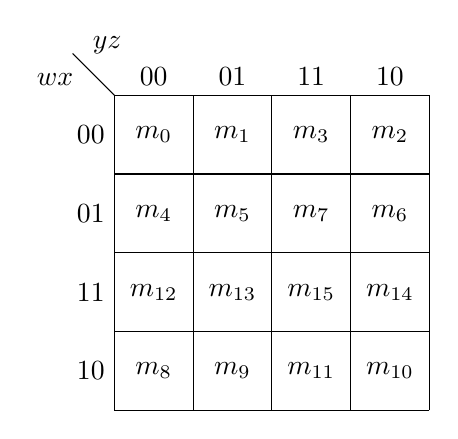
\begin{tikzpicture}
\pgfmathsetmacro{\kxstep}{1}
\pgfmathsetmacro{\kystep}{1}
\pgfmathsetmacro{\kpin}{0.75}
\draw[xstep=\kxstep,ystep=\kystep](0,0) grid (4*\kxstep,-4*\kystep);
\draw(0,0)--++(135:\kpin)node[pos=0.75,above right]{$yz$}node[pos=0.75,below left]{$wx$};
\foreach \kx/\xlb in {0/{00},1/{01},2/{11},3/{10}}{\draw(\kx*\kxstep+\kxstep/2,0)node[above]{$\xlb$};}
\foreach \ky/\ylb in {0/{00},1/{01},2/{11},3/{10}}{\draw(0,-\ky*\kystep-\kystep/2)node[left]{$\ylb$};}
\foreach \kx/\xlb in {0/{m_0},1/{m_1},2/{m_3},3/{m_2}}{\draw(\kx*\kxstep+\kxstep/2,-\kystep/2)node[]{$\xlb$};}
\foreach \kx/\xlb in {0/{m_4},1/{m_5},2/{m_7},3/{m_6}}{\draw(\kx*\kxstep+\kxstep/2,-1.5*\kystep)node[]{$\xlb$};}
\foreach \kx/\xlb in {0/{m_{12}},1/{m_{13}},2/{m_{15}},3/{m_{14}}}{\draw(\kx*\kxstep+\kxstep/2,-2.5*\kystep)node[]{$\xlb$};}
\foreach \kx/\xlb in {0/{m_8},1/{m_9},2/{m_{11}},3/{m_{10}}}{\draw(\kx*\kxstep+\kxstep/2,-3.5*\kystep)node[]{$\xlb$};}
\end{tikzpicture}
\caption{چار متغیر کارناف نقشے کی بنیادی صورت۔}
\label{شکل_کارناف_چار_متغیر_بنیادی_صورت}
\end{figure}

اب تک آپ پر واضح ہو چکا ہو گا کہ کارناف نقشے بناتے ہوئے صفوں اور قطاروں کو\قول{ \, گرے رمز } میں میں رکھا جاتا ہے۔چار سے زیادہ متغیرات کے کارناف نقشوں کا استعمال نسبتاً پیچیدہ ہوتا ہے، لہٰذا ان سے تفاعل کا سادہ روپ عموماً کمپیوٹر کی مدد سے حاصل کیا جاتا ہے۔ 


\حصہ{کارناف نقشے کی بھرائی}
 بوولین جدول سے کارناف نقشے کی بھرائی نہایت آسان اور سیدھا عمل ہے۔بوولین جدول کی جن صفوں میں تفاعل کی قیمت \عددی{1} ہو، ان کے مطابقتی (کارناف نقشہ کے) خانوں میں \عددی{1} پُر کریں؛ باقی خانوں میں \عددی{0} پُر کریں۔شکل \حوالہ{شکل_کارناف_دو_بھرائی}-الف میں دو آزاد متغیر تفاعل \عددی{F=\sum (m_0,m_1)} کے لئے یہ عمل دکھایا گیا ہے۔شکل-ج میں تفاعل کا کارناف کا نقشہ پُر کیا ہوا دکھایا گیا ہے۔ تفاعل کو مجموعہ ارکان ضرب کے روپ میں لکھنے سے کارناف نقشہ میں پُر کئے جانے والے خانوں کی نشاندہی ہوتی ہے۔
 
\begin{figure}
\centering
\begin{subfigure}{1\textwidth}
\centering
\begin{otherlanguage}{english}
\begin{tabular}{CC|C|C}
\toprule
x&y&F&\text{\RL{ارکان ضرب}}\\
\midrule
0&0&1&m_0\\
0&1&1&m_1\\
1&0&0&m_2\\
1&1&0&m_3\\
\bottomrule
\end{tabular}\quad\quad
\begin{tikzpicture}
$F=\sum(m_0,m_1)$
\end{tikzpicture}
\end{otherlanguage}
\caption{}
\end{subfigure}\hfill
\begin{subfigure}{0.45\textwidth}
\centering
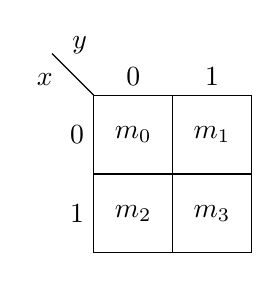
\begin{tikzpicture}
\pgfmathsetmacro{\kxstep}{1}
\pgfmathsetmacro{\kystep}{1}
\pgfmathsetmacro{\kpin}{0.75}
\draw[xstep=\kxstep,ystep=\kystep](0,0) grid (2*\kxstep,-2*\kystep);
\draw(0,0)--++(135:\kpin)node[pos=0.75,above right]{$y$}node[pos=0.75,below left]{$x$};
\foreach \kx/\xlb in {0/{0},1/{1}}{\draw(\kx*\kxstep+\kxstep/2,0)node[above]{$\xlb$};}
\foreach \ky/\ylb in {0/0,1/1}{\draw(0,-\ky*\kystep-\kystep/2)node[left]{$\ylb$};}
\foreach \kx/\xlb in {0/{m_0},1/{m_1}}{\draw(\kx*\kxstep+\kxstep/2,-\kystep/2)node[]{$\xlb$};}
\foreach \kx/\xlb in {0/{m_2},1/{m_3}}{\draw(\kx*\kxstep+\kxstep/2,-1.5*\kystep)node[]{$\xlb$};}
\end{tikzpicture}
\caption{}
\end{subfigure}\hfill
\begin{subfigure}{0.45\textwidth}
\centering
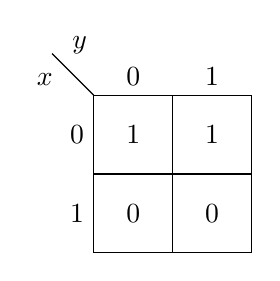
\begin{tikzpicture}
\pgfmathsetmacro{\kxstep}{1}
\pgfmathsetmacro{\kystep}{1}
\pgfmathsetmacro{\kpin}{0.75}
\draw[xstep=\kxstep,ystep=\kystep](0,0) grid (2*\kxstep,-2*\kystep);
\draw(0,0)--++(135:\kpin)node[pos=0.75,above right]{$y$}node[pos=0.75,below left]{$x$};
\foreach \kx/\xlb in {0/{0},1/{1}}{\draw(\kx*\kxstep+\kxstep/2,0)node[above]{$\xlb$};}
\foreach \ky/\ylb in {0/0,1/1}{\draw(0,-\ky*\kystep-\kystep/2)node[left]{$\ylb$};}
\foreach \kx/\xlb in {0/{1},1/{1}}{\draw(\kx*\kxstep+\kxstep/2,-\kystep/2)node[]{$\xlb$};}
\foreach \kx/\xlb in {0/{0},1/{0}}{\draw(\kx*\kxstep+\kxstep/2,-1.5*\kystep)node[]{$\xlb$};}
\end{tikzpicture}
\caption{}
\end{subfigure}
\caption{دو متغیر تفاعل کارناف نقشے کی بھرائی۔}
\label{شکل_کارناف_دو_بھرائی}
\end{figure}

تین آزاد متغیر تفاعل \عددی{F=\sum (m_3,m_5,m_6,m_7)} کی مثال شکل \حوالہ{شکل_کارناف_تین_بھرائی} میں پیش کی گئی ہیں۔

\begin{figure}
\centering
\begin{subfigure}{1\textwidth}
\centering
\begin{otherlanguage}{english}
\begin{tabular}{CCC|C|C}
\toprule
x&y&z&F&\text{\RL{ارکان ضرب}}\\
\midrule
0&0&0&0&m_0\\
0&0&1&0&m_1\\
0&1&0&0&m_2\\
0&1&1&1&m_3\\
1&0&0&0&m_4\\
1&0&1&1&m_5\\
1&1&0&1&m_6\\
1&1&1&1&m_7\\
\bottomrule
\end{tabular}\quad\quad
\begin{tikzpicture}
$F=\sum(m_3, m_5, m_6, m_7)$
\end{tikzpicture}
\end{otherlanguage}
\caption{}
\end{subfigure}
\begin{subfigure}{0.45\textwidth}
\centering
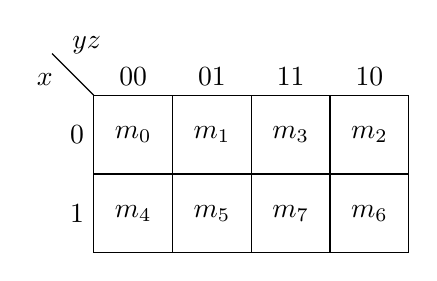
\begin{tikzpicture}
\pgfmathsetmacro{\kxstep}{1}
\pgfmathsetmacro{\kystep}{1}
\pgfmathsetmacro{\kpin}{0.75}
\draw[xstep=\kxstep,ystep=\kystep](0,0) grid (4*\kxstep,-2*\kystep);
\draw(0,0)--++(135:\kpin)node[pos=0.75,above right]{$yz$}node[pos=0.75,below left]{$x$};
\foreach \kx/\xlb in {0/{00},1/{01},2/{11},3/{10}}{\draw(\kx*\kxstep+\kxstep/2,0)node[above]{$\xlb$};}
\foreach \ky/\ylb in {0/0,1/1}{\draw(0,-\ky*\kystep-\kystep/2)node[left]{$\ylb$};}
\foreach \kx/\xlb in {0/{m_0},1/{m_1},2/{m_3},3/{m_2}}{\draw(\kx*\kxstep+\kxstep/2,-\kystep/2)node[]{$\xlb$};}
\foreach \kx/\xlb in {0/{m_4},1/{m_5},2/{m_7},3/{m_6}}{\draw(\kx*\kxstep+\kxstep/2,-1.5*\kystep)node[]{$\xlb$};}
\end{tikzpicture}
\caption{}
\end{subfigure}\hfill
\begin{subfigure}{0.45\textwidth}
\centering
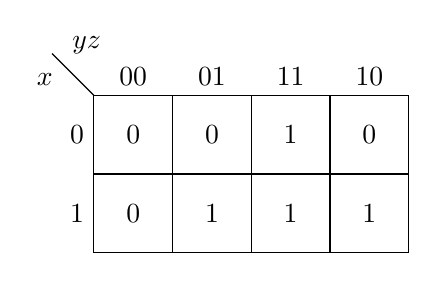
\begin{tikzpicture}
\pgfmathsetmacro{\kxstep}{1}
\pgfmathsetmacro{\kystep}{1}
\pgfmathsetmacro{\kpin}{0.75}
\draw[xstep=\kxstep,ystep=\kystep](0,0) grid (4*\kxstep,-2*\kystep);
\draw(0,0)--++(135:\kpin)node[pos=0.75,above right]{$yz$}node[pos=0.75,below left]{$x$};
\foreach \kx/\xlb in {0/{00},1/{01},2/{11},3/{10}}{\draw(\kx*\kxstep+\kxstep/2,0)node[above]{$\xlb$};}
\foreach \ky/\ylb in {0/0,1/1}{\draw(0,-\ky*\kystep-\kystep/2)node[left]{$\ylb$};}
\foreach \kx/\xlb in {0/{0},1/{0},2/{1},3/{0}}{\draw(\kx*\kxstep+\kxstep/2,-\kystep/2)node[]{$\xlb$};}
\foreach \kx/\xlb in {0/{0},1/{1},2/{1},3/{1}}{\draw(\kx*\kxstep+\kxstep/2,-1.5*\kystep)node[]{$\xlb$};}
\end{tikzpicture}
\caption{}
\end{subfigure}
\caption{تین متغیر کارناف نقشے کی بھرائی۔}
\label{شکل_کارناف_تین_بھرائی}
\end{figure}



\حصہ{کارناف نقشے سے تفاعل کی سادہ مساوات کا حصول}
کارناف نقشے میں قریبی خانوں سے مراد ایسے \عددی{2^n} خانے ہیں جنہیں مربع یا مستطیل میں گھیرا جا سکے؛ یہاں \عددی{n} کی قیمت \عددی{1}، \عددی{2}، \عددی{3}، وغیرہ ہو سکتی ہے۔یوں \عددی{2}، \عددی{4}، \عددی{8}،وغیرہ ، ایسے خانے جنہیں مربع یا مستطیل میں گھیرا جا سکے قریبی خانے کہلائیں گے۔کوئی بھی خانہ (یا خانے) ایک سے زیادہ مربع یا مستطیل کا حصہ بن سکتا ہے (سکتے ہیں)۔

قریبی خانوں میں تفاعل کی قیمت \عددی{1} ہونے کی صورت میں، ان خانوں کے ارکان ضرب کا مجموعہ بوولین قوانین سے حل کر کے سادہ ترین رکن ضرب حاصل کیا جا سکتا ہے۔یہ رکن ان قریبی خانوں کے ارکان ضرب میں مشترک حصے پر مشتمل ہو گا۔

دو قریبی بلند خانوں (جن میں تفاعل کی قیمت \عددی{1} ہو گی، کے ارکان ضرب کے مجموعہ ) سے حاصل، سادہ ترین رکن ضرب میں آزاد متغیرات کی تعداد، تفاعل میں آزاد متغیرات کی تعداد سے ایک کم ہو گی۔اسی طرح، چار بلند قریبی خانوں سے حاصل، سادہ ترین رکن ضرب میں آزاد متغیرات کی تعداد، تفاعل میں آزاد متغیرات کی تعداد سے دو کم ہو گی۔آٹھ قریبی بلند خانوں سے حاصل، سادہ ترین رکن ضرب میں آزاد متغیرات کی تعداد، تفاعل میں آزاد متغیرات کی تعداد سے چار کم ہو گی۔
	
قریبی خانے گھیرتے وقت یہ کوشش ہونی چاہئے کہ بڑے سے بڑا مربع یا مستطیل بنے۔ایسا کرنے سے سادہ ترین رکن ضرب حاصل ہو گا۔عموماً، قریبی خانوں کو ایک سے زیادہ طریقوں سے گھیرا جا سکتا ہے، جن سے تفاعل کی مختلف سادہ صورتیں حاصل ہوں گی۔
	
اب ہم چند مثالوں کی مدد سے اس طریقہ کار کو سیکھتے ہیں۔
	

\جزوحصہ{دو آزاد متغیر تفاعل}
دو متغیر تفاعل کے کارناف نقشہ میں \عددی{m_0} اور \عددی{m_1} قریبی خانے ہوں گے۔اسی طرح \عددی{m_0} اور \عددی{m_2} بھی قریبی خانے ہوں گے، جبکہ \عددی{m_1} اور \عددی{m_2} قریبی خانے نہیں ہوں گے۔

شکل \حوالہ{شکل_کارناف_قریبی_سادہ} میں دو متغیر تفاعل اور اس کا کارناف نقشہ دیا گیا ہے۔ کارناف نقشے میں خانوں سے اوپر، متغیر \عددی{y} کی ممکن قیمتوں \عددی{0} اور \عددی{1} کی بجائے بالترتیب \عددی{\overline{y}} اور \عددی{y} لکھا گیا ہے (یعنی \عددی{1} کی جگہ متغیر لکھا گیا ہے جبکہ \عددی{0} کی جگہ متغیر لکھ کر اس پر لکیر لگائی گئی ہے جو پست متغیر کو ظاہر کرتا ہے)۔ اسی طرح خانوں کے بائیں جانب \عددی{\overline{x}} اور \عددی{x} لکھا گیا ہے۔

 کارناف نقشے کے دو قریبی خانوں میں تفاعل کی قیمت \عددی{1} ہے، جنہیں نقطہ دار مستطیل میں گھیرا گیا ہے۔شکل-د میں ان خانوں کے ارکان ضرب کے مجموعے کو بوولین قوانین سے حل کر کے سادہ رکن حاصل کیا گیا۔آپ دیکھ سکتے ہیں کہ ان خانوں کے ارکان ضرب کے مجموعے سے ایک متغیر رکن حاصل ہوتا ہے؛ یعنی دو متغیر تفاعل کی صورت میں دو خانوں سے ایک متغیر رکن حاصل ہوا۔

یہی مساوات، شکل-ج کے کارناف نقشے میں نقطہ دار مستطیل میں گھیرے ، دو قریبی خانوں کو دیکھ کر لکھی جا سکتی ہے۔نقطہ دار مستطیل میں گھیرے دو قریبی خانوں کے ارکان ضرب \عددی{\overline{x}\,\overline{y}} اور \عددی{\overline{x}y} ہیں۔ ان ارکان ضرب میں \عددی{\overline{x}} مشترک ہے، جبکہ ایک رکن میں \عددی{\overline{y}} اور دوسرے میں \عددی{y} ہے۔ یوں، نقطہ دار مستطیل میں گھیرے ارکان ضرب میں وہ حصہ جو مشترک ہو مطلوبہ سادہ رکن ہو گا۔ ( غیر مشترک حصہ رد کرنا، شکل-د میں \عددی{\overline{y}+y=1} کے مترادف ہے۔) چونکہ ان خانوں کے علاوہ تمام خانوں میں \عددی{0} ہے لہٰذا یہی رکن تفاعل کی مساوات \عددی{(F=\overline{x})} ہو گی۔

\begin{figure}
\centering
\begin{subfigure}{0.25\textwidth}
\centering
\begin{otherlanguage}{english}
\begin{tabular}{CC|C|C}
\toprule
x&y&F&\\
\midrule
0&0&1&m_0\\
0&1&1&m_1\\
1&0&0&m_2\\
1&1&0&m_3\\
\bottomrule
\end{tabular}
\end{otherlanguage}
\caption{}
\end{subfigure}\hfill
\begin{subfigure}{0.25\textwidth}
\centering
\begin{tikzpicture}
\pgfmathsetmacro{\kxstep}{1}
\pgfmathsetmacro{\kystep}{1}
\pgfmathsetmacro{\kpin}{0.75}
\pgfmathsetmacro{\kmv}{0.15}
\draw[xstep=\kxstep,ystep=\kystep](0,0) grid (2*\kxstep,-2*\kystep);
%\draw(0,0)--++(135:\kpin)node[pos=0.75,above right]{$y$}node[pos=0.75,below left]{$x$};
\foreach \kx/\xlb in {0/{\overline{y}},1/{y}}{\draw(\kx*\kxstep+\kxstep/2,0)node[above]{$\xlb$};}
\foreach \ky/\ylb in {0/{\overline{x}},1/{x}}{\draw(0,-\ky*\kystep-\kystep/2)node[left]{$\ylb$};}
\foreach \kx/\xlb in {0/{1},1/{1}}{\draw(\kx*\kxstep+\kxstep/2,-\kystep/2)node[]{$\xlb$};}
\foreach \kx/\xlb in {0/{0},1/{0}}{\draw(\kx*\kxstep+\kxstep/2,-1.5*\kystep)node[]{$\xlb$};}
\draw[gray,dashed] ($(0,0)+(\kmv,-\kmv)$) rectangle ($(2*\kxstep,-\kystep)+(-\kmv,\kmv)$);
\end{tikzpicture}
\caption{}
\end{subfigure}\hfill
\begin{subfigure}{0.25\textwidth}
\centering
\begin{tikzpicture}
\pgfmathsetmacro{\kxstep}{1}
\pgfmathsetmacro{\kystep}{1}
\pgfmathsetmacro{\kpin}{0.75}
\pgfmathsetmacro{\kmv}{0.15}
\draw[xstep=\kxstep,ystep=\kystep](0,0) grid (2*\kxstep,-2*\kystep);
%\draw(0,0)--++(135:\kpin)node[pos=0.75,above right]{$yz$}node[pos=0.75,below left]{$x$};
\foreach \kx/\xlb in {0/{\overline{y}},1/{y}}{\draw(\kx*\kxstep+\kxstep/2,0)node[above]{$\xlb$};}
\foreach \ky/\ylb in {0/{\overline{x}},1/{x}}{\draw(0,-\ky*\kystep-\kystep/2)node[left]{$\ylb$};}
\foreach \kx/\xlb in {0/{\overline{x}\,\overline{y}},1/{\overline{x}y}}{\draw(\kx*\kxstep+\kxstep/2,-\kystep/2)node[]{$\xlb$};}
%\foreach \kx/\xlb in {0/{0},1/{0}}{\draw(\kx*\kxstep+\kxstep/2,-1.5*\kystep)node[]{$\xlb$};}
\draw[gray,dashed] ($(0,0)+(\kmv,-\kmv)$) rectangle ($(2*\kxstep,-\kystep)+(-\kmv,\kmv)$);
\end{tikzpicture}
\caption{}
\end{subfigure}\hfill
\begin{subfigure}{0.25\textwidth}
\centering
\begin{tikzpicture}
\draw(0,0)node[]{$\begin{aligned}
F&=\overline{x}\,\overline{y}+\overline{x}y\\
&=\overline{x}(\overline{y}+y)\\
&=\overline{x}(1)\\
&=\overline{x}
\end{aligned}$};
\end{tikzpicture}
\caption{}
\end{subfigure}
\caption{قریبی بلند خانوں سے سادہ رکن ضرب کا حصول۔}
\label{شکل_کارناف_قریبی_سادہ}
\end{figure}
	


شکل \حوالہ{شکل_کارناف_قریبی_پہلا_مزید} میں ایک تفاعل کا جدول دیا گیا ہے جس قریبی خانوں کے ارکان ضرب \عددی{\overline{x}\,\overline{y}} اور \عددی{x\overline{y}} میں \عددی{\overline{y}} مشترک ہے۔چونکہ باقی خانوں میں \عددی{0} ہے، لہٰذا اس تفاعل کی سادہ مساوات \عددی{F=\overline{y}} ہو گی۔

\begin{figure}
\centering
\begin{subfigure}{0.30\textwidth}
\centering
\begin{tikzpicture}
\pgfmathsetmacro{\kxstep}{1}
\pgfmathsetmacro{\kystep}{1}
\pgfmathsetmacro{\kpin}{0.75}
\pgfmathsetmacro{\kmv}{0.15}
\draw[xstep=\kxstep,ystep=\kystep](0,0) grid (2*\kxstep,-2*\kystep);
%\draw(0,0)--++(135:\kpin)node[pos=0.75,above right]{$y$}node[pos=0.75,below left]{$x$};
\foreach \kx/\xlb in {0/{\overline{y}},1/{y}}{\draw(\kx*\kxstep+\kxstep/2,0)node[above]{$\xlb$};}
\foreach \ky/\ylb in {0/{\overline{x}},1/{x}}{\draw(0,-\ky*\kystep-\kystep/2)node[left]{$\ylb$};}
\foreach \kx/\xlb in {0/{1},1/{0}}{\draw(\kx*\kxstep+\kxstep/2,-\kystep/2)node[]{$\xlb$};}
\foreach \kx/\xlb in {0/{1},1/{0}}{\draw(\kx*\kxstep+\kxstep/2,-1.5*\kystep)node[]{$\xlb$};}
\draw[gray,dashed] ($(0,0)+(\kmv,-\kmv)$) rectangle ($(\kxstep,-2*\kystep)+(-\kmv,\kmv)$);
\end{tikzpicture}
\caption{}
\end{subfigure}\hfill
\begin{subfigure}{0.30\textwidth}
\centering
\begin{tikzpicture}
\pgfmathsetmacro{\kxstep}{1}
\pgfmathsetmacro{\kystep}{1}
\pgfmathsetmacro{\kpin}{0.75}
\pgfmathsetmacro{\kmv}{0.15}
\draw[xstep=\kxstep,ystep=\kystep](0,0) grid (2*\kxstep,-2*\kystep);
%\draw(0,0)--++(135:\kpin)node[pos=0.75,above right]{$yz$}node[pos=0.75,below left]{$x$};
\foreach \kx/\xlb in {0/{\overline{y}},1/{y}}{\draw(\kx*\kxstep+\kxstep/2,0)node[above]{$\xlb$};}
\foreach \ky/\ylb in {0/{\overline{x}},1/{x}}{\draw(0,-\ky*\kystep-\kystep/2)node[left]{$\ylb$};}
\foreach \kx/\xlb in {0/{\overline{x}\,\overline{y}}}{\draw(\kx*\kxstep+\kxstep/2,-\kystep/2)node[]{$\xlb$};}
\foreach \kx/\xlb in {0/{x\overline{y}}}{\draw(\kx*\kxstep+\kxstep/2,-1.5*\kystep)node[]{$\xlb$};}
\draw[gray,dashed] ($(0,0)+(\kmv,-\kmv)$) rectangle ($(\kxstep,-2*\kystep)+(-\kmv,\kmv)$);
\end{tikzpicture}
\caption{}
\end{subfigure}\hfill
\begin{subfigure}{0.30\textwidth}
\centering
\begin{tikzpicture}
\draw(0,0)node[]{$\begin{aligned}
F&=\overline{x}\,\overline{y}+x\overline{y}\\
&=(\overline{x}+x)\overline{y}\\
&=(1)\overline{y}\\
&=\overline{y}
\end{aligned}$};
\end{tikzpicture}
\caption{}
\end{subfigure}
\caption{قریبی بلند خانوں سے سادہ رکن ضرب کا حصول۔}
\label{شکل_کارناف_قریبی_پہلا_مزید}
\end{figure}

شکل \حوالہ{شکل_کارناف_قریبی_دوسرا_مزید} کے تفاعل کے ارکان ضرب \عددی{x\overline{y}} اور \عددی{xy} میں \عددی{x} مشترک ہے (شکل-ج دیکھیں)۔چونکہ باقی خانوں میں تفاعل کی قیمت \عددی{0} ہے لہٰذا تفاعل کے ارکان ضرب کا مجموعہ اسی رکن کے برابر ہو گا۔ یوں اس کی مساوات \عددی{F=x} ہو گی۔

\begin{figure}
\centering
\begin{subfigure}{0.30\textwidth}
\centering
\begin{tikzpicture}
\pgfmathsetmacro{\kxstep}{1}
\pgfmathsetmacro{\kystep}{1}
\pgfmathsetmacro{\kpin}{0.75}
\pgfmathsetmacro{\kmv}{0.15}
\draw[xstep=\kxstep,ystep=\kystep](0,0) grid (2*\kxstep,-2*\kystep);
%\draw(0,0)--++(135:\kpin)node[pos=0.75,above right]{$y$}node[pos=0.75,below left]{$x$};
\foreach \kx/\xlb in {0/{\overline{y}},1/{y}}{\draw(\kx*\kxstep+\kxstep/2,0)node[above]{$\xlb$};}
\foreach \ky/\ylb in {0/{\overline{x}},1/{x}}{\draw(0,-\ky*\kystep-\kystep/2)node[left]{$\ylb$};}
\foreach \kx/\xlb in {0/{0},1/{0}}{\draw(\kx*\kxstep+\kxstep/2,-\kystep/2)node[]{$\xlb$};}
\foreach \kx/\xlb in {0/{1},1/{1}}{\draw(\kx*\kxstep+\kxstep/2,-1.5*\kystep)node[]{$\xlb$};}
\draw[gray,dashed] ($(0,-\kystep)+(\kmv,-\kmv)$) rectangle ($(2*\kxstep,-2*\kystep)+(-\kmv,\kmv)$);
\end{tikzpicture}
\caption{}
\end{subfigure}\hfill
\begin{subfigure}{0.30\textwidth}
\centering
\begin{tikzpicture}
\pgfmathsetmacro{\kxstep}{1}
\pgfmathsetmacro{\kystep}{1}
\pgfmathsetmacro{\kpin}{0.75}
\pgfmathsetmacro{\kmv}{0.15}
\draw[xstep=\kxstep,ystep=\kystep](0,0) grid (2*\kxstep,-2*\kystep);
%\draw(0,0)--++(135:\kpin)node[pos=0.75,above right]{$yz$}node[pos=0.75,below left]{$x$};
\foreach \kx/\xlb in {0/{\overline{y}},1/{y}}{\draw(\kx*\kxstep+\kxstep/2,0)node[above]{$\xlb$};}
\foreach \ky/\ylb in {0/{\overline{x}},1/{x}}{\draw(0,-\ky*\kystep-\kystep/2)node[left]{$\ylb$};}
%\foreach \kx/\xlb in {0/{\overline{x}\,\overline{y}}}{\draw(\kx*\kxstep+\kxstep/2,-\kystep/2)node[]{$\xlb$};}
\foreach \kx/\xlb in {0/{x\overline{y}},1/{xy}}{\draw(\kx*\kxstep+\kxstep/2,-1.5*\kystep)node[]{$\xlb$};}
\draw[gray,dashed] ($(0,-\kystep)+(\kmv,-\kmv)$) rectangle ($(2*\kxstep,-2*\kystep)+(-\kmv,\kmv)$);
\end{tikzpicture}
\caption{}
\end{subfigure}\hfill
\begin{subfigure}{0.30\textwidth}
\centering
\begin{tikzpicture}
%\draw[step=1,thick](-2,-2) grid (2,1);
%\draw[step=0.1,gray](-2,-2) grid (2,1);
\draw(0,0) node[]{$x\overline{y}, \quad xy$};
\draw[gray](-0.5,-0.2)--++(0,-0.1)--(0.5,-0.5) (0.3,-0.2)--++(0,-0.1)--(0.5,-0.5)node[black,below,xshift=-2em]{\text{\RL{لکھائی میں \عددی{x} مشترک ہے}}};
\draw[gray](-0.3,0.2)--++(0,0.1)--(-1,0.5) (0.5,0.2)--++(0,0.1)--(-1,0.5)node[black,above]{\text{\RL{یہ دو مختلف ہیں}}};
\end{tikzpicture}
\caption{}
\end{subfigure}
\caption{قریبی بلند خانوں سے سادہ رکن ضرب کا حصول۔}
\label{شکل_کارناف_قریبی_دوسرا_مزید}
\end{figure}



شکل \حوالہ{شکل_کارناف_قریبی_تیسرا_مزید} میں ایک ہی خانے کو دو قریبی خانوں کے ساتھ باری باری جوڑتے ہوئے سادہ مساوات \عددی{(F=\overline{x}+\overline{y})} حاصل کرنا دکھایا گیا ہے۔آئیں اس مساوات کو بوولین منطق کی مدد سے حاصل کریں۔مساوات کو ارکان ضرب کا مجموعہ لکھ کر اس کی سادہ روپ اخذ کرتے ہیں:
\begin{align*}
F&=x\overline{y}+\overline{x}\,\overline{y}+\overline{x}y\\
&=x\overline{y}+\overline{x}\,\overline{y}+\overline{x}\,\overline{y}+\overline{x}y\\
&=(x+\overline{x})\overline{y}+\overline{x}(\overline{y}+y)\\
&=(1)\overline{y}+\overline{x}(1)\\
&=\overline{y}+\overline{x}
\end{align*}

 جہاں، دوسرے قدم پر جدول \حوالہ{جدول_بوولین_دو_پہلو_تفاعل}-ب کی شِق \عددی{4} (صفحہ \حوالہصفحہ{جدول_بوولین_دو_پہلو_تفاعل}) استعمال کرتے
 ہوئے \عددی{\overline{x}\,\overline{y}=\overline{x}\,\overline{y}+\overline{x}\,\overline{y}} لکھا گیا۔

\begin{figure}
\centering
\begin{subfigure}{0.30\textwidth}
\centering
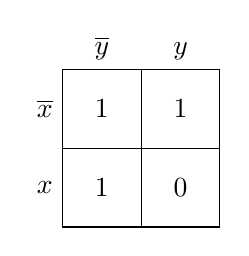
\begin{tikzpicture}
\pgfmathsetmacro{\kxstep}{1}
\pgfmathsetmacro{\kystep}{1}
\pgfmathsetmacro{\kpin}{0.75}
\pgfmathsetmacro{\kmv}{0.15}
\draw[xstep=\kxstep,ystep=\kystep](0,0) grid (2*\kxstep,-2*\kystep);
%\draw(0,0)--++(135:\kpin)node[pos=0.75,above right]{$y$}node[pos=0.75,below left]{$x$};
\foreach \kx/\xlb in {0/{\overline{y}},1/{y}}{\draw(\kx*\kxstep+\kxstep/2,0)node[above]{$\xlb$};}
\foreach \ky/\ylb in {0/{\overline{x}},1/{x}}{\draw(0,-\ky*\kystep-\kystep/2)node[left]{$\ylb$};}
\foreach \kx/\xlb in {0/{1},1/{1}}{\draw(\kx*\kxstep+\kxstep/2,-\kystep/2)node[]{$\xlb$};}
\foreach \kx/\xlb in {0/{1},1/{0}}{\draw(\kx*\kxstep+\kxstep/2,-1.5*\kystep)node[]{$\xlb$};}
%\draw[gray,dashed] ($(0,-\kystep)+(\kmv,-\kmv)$) rectangle ($(2*\kxstep,-2*\kystep)+(-\kmv,\kmv)$);
\end{tikzpicture}
\end{subfigure}\hfill
\begin{subfigure}{0.30\textwidth}
\centering
\begin{tikzpicture}
\pgfmathsetmacro{\kxstep}{1}
\pgfmathsetmacro{\kystep}{1}
\pgfmathsetmacro{\kpin}{0.75}
\pgfmathsetmacro{\kmv}{0.15}
\pgfmathsetmacro{\kmva}{0.1}
\draw[xstep=\kxstep,ystep=\kystep](0,0) grid (2*\kxstep,-2*\kystep);
%\draw(0,0)--++(135:\kpin)node[pos=0.75,above right]{$yz$}node[pos=0.75,below left]{$x$};
\foreach \kx/\xlb in {0/{\overline{y}},1/{y}}{\draw(\kx*\kxstep+\kxstep/2,0)node[above]{$\xlb$};}
\foreach \ky/\ylb in {0/{\overline{x}},1/{x}}{\draw(0,-\ky*\kystep-\kystep/2)node[left]{$\ylb$};}
\foreach \kx/\xlb in {0/{\overline{x}\,\overline{y}},1/{\overline{x}y}}{\draw(\kx*\kxstep+\kxstep/2,-\kystep/2)node[]{$\xlb$};}
\foreach \kx/\xlb in {0/{x\overline{y}}}{\draw(\kx*\kxstep+\kxstep/2,-1.5*\kystep)node[]{$\xlb$};}
\draw[gray,dashed] ($(0,0)+(\kmv,-\kmv)$) rectangle ($(2*\kxstep,-1*\kystep)+(-\kmv,\kmv)$);
\draw[gray,dashed] ($(0,0)+(\kmva,-\kmva)$) rectangle ($(1*\kxstep,-2*\kystep)+(-\kmva,\kmva)$);
\end{tikzpicture}
\end{subfigure}\hfill
\begin{subfigure}{0.40\textwidth}
\centering
\begin{tikzpicture}
%\draw[step=1,thick](-2,-2) grid (2,1);
%\draw[step=0.1,gray](-2,-2) grid (2,1);
\draw(0,0) node[]{\text{\RL{
\عددی{\overline{x}\,\overline{y}} اور \عددی{\overline{x}y} لکھنے میں \عددی{\overline{x}} مشترک ہے،
}}};
\draw(0,-0.75) node[]{\text{\RL{
\عددی{\overline{x}\,\overline{y}} اور \عددی{x\overline{y}} لکھنے میں \عددی{\overline{y}} مشترک ہے،
}}};
\draw(0,-1.5) node[]{\text{\RL{
لہٰذا مساوات \عددی{F=\overline{x}+\overline{y}} ہو گی۔
}}};
\end{tikzpicture}
\end{subfigure}
\caption{قریبی بلند خانوں سے سادہ رکن کا حصول۔}
\label{شکل_کارناف_قریبی_تیسرا_مزید}
\end{figure}

شکل \حوالہ{شکل_کارناف_قریبی_چوتھا_مزید} میں چار قریبی خانے ایک مستطیل میں گھیرے جا سکتے ہیں۔ ایسی صورت میں تفاعل ہمیشہ بلند \عددی{(1)} رہے گا لہٰذا اس کی مساوات \عددی{F=1} ہو گی۔
\begin{figure}
\centering
\begin{subfigure}{0.40\textwidth}
\centering
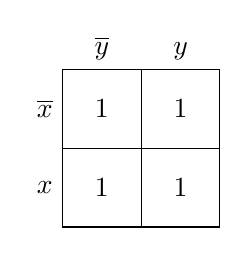
\begin{tikzpicture}
\pgfmathsetmacro{\kxstep}{1}
\pgfmathsetmacro{\kystep}{1}
\pgfmathsetmacro{\kpin}{0.75}
\pgfmathsetmacro{\kmv}{0.15}
\draw[xstep=\kxstep,ystep=\kystep](0,0) grid (2*\kxstep,-2*\kystep);
%\draw(0,0)--++(135:\kpin)node[pos=0.75,above right]{$y$}node[pos=0.75,below left]{$x$};
\foreach \kx/\xlb in {0/{\overline{y}},1/{y}}{\draw(\kx*\kxstep+\kxstep/2,0)node[above]{$\xlb$};}
\foreach \ky/\ylb in {0/{\overline{x}},1/{x}}{\draw(0,-\ky*\kystep-\kystep/2)node[left]{$\ylb$};}
\foreach \kx/\xlb in {0/{1},1/{1}}{\draw(\kx*\kxstep+\kxstep/2,-\kystep/2)node[]{$\xlb$};}
\foreach \kx/\xlb in {0/{1},1/{1}}{\draw(\kx*\kxstep+\kxstep/2,-1.5*\kystep)node[]{$\xlb$};}
%\draw[gray,dashed] ($(0,-\kystep)+(\kmv,-\kmv)$) rectangle ($(2*\kxstep,-2*\kystep)+(-\kmv,\kmv)$);
\end{tikzpicture}
\end{subfigure}\hfill
\begin{subfigure}{0.40\textwidth}
\centering
\begin{tikzpicture}
\pgfmathsetmacro{\kxstep}{1}
\pgfmathsetmacro{\kystep}{1}
\pgfmathsetmacro{\kpin}{0.75}
\pgfmathsetmacro{\kmv}{0.15}
\pgfmathsetmacro{\kmva}{0.1}
\draw[xstep=\kxstep,ystep=\kystep](0,0) grid (2*\kxstep,-2*\kystep);
%\draw(0,0)--++(135:\kpin)node[pos=0.75,above right]{$yz$}node[pos=0.75,below left]{$x$};
\foreach \kx/\xlb in {0/{\overline{y}},1/{y}}{\draw(\kx*\kxstep+\kxstep/2,0)node[above]{$\xlb$};}
\foreach \ky/\ylb in {0/{\overline{x}},1/{x}}{\draw(0,-\ky*\kystep-\kystep/2)node[left]{$\ylb$};}
\foreach \kx/\xlb in {0/{\overline{x}\,\overline{y}},1/{\overline{x}y}}{\draw(\kx*\kxstep+\kxstep/2,-\kystep/2)node[]{$\xlb$};}
\foreach \kx/\xlb in {0/{x\overline{y}},1/{xy}}{\draw(\kx*\kxstep+\kxstep/2,-1.5*\kystep)node[]{$\xlb$};}
\draw[gray,dashed] ($(0,0)+(\kmv,-\kmv)$) rectangle ($(2*\kxstep,-2*\kystep)+(-\kmv,\kmv)$);
\end{tikzpicture}
\end{subfigure}\hfill
\begin{subfigure}{0.20\textwidth}
\centering
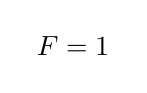
\begin{tikzpicture}
%\draw[step=1,thick](-2,-2) grid (2,1);
%\draw[step=0.1,gray](-2,-2) grid (2,1);
\draw(0,0) node[]{$F=1$};
\end{tikzpicture}
\end{subfigure}
\caption{چار قریبی خانوں سے سادہ رکن \عددی{1} حاصل ہو گا۔}
\label{شکل_کارناف_قریبی_چوتھا_مزید}
\end{figure}

شکل \حوالہ{شکل_کارناف_قریبی_پانچ_مزید} میں قریبی خانے نہیں پائے جاتے، لہٰذا ارکان ضرب کے مجموعہ کو مزید سادہ نہیں بنایا جا سکتا۔ جب بھی کوئی خانہ کسی مستطیل میں شامل نہ ہو، اس کا رکن ضرب جوں کا توں مجموعہ (اور مساوات) میں رہے گا۔ 

\begin{figure}
\centering
\begin{subfigure}{0.30\textwidth}
\centering
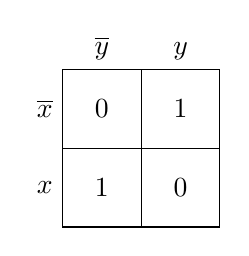
\begin{tikzpicture}
\pgfmathsetmacro{\kxstep}{1}
\pgfmathsetmacro{\kystep}{1}
\pgfmathsetmacro{\kpin}{0.75}
\pgfmathsetmacro{\kmv}{0.15}
\draw[xstep=\kxstep,ystep=\kystep](0,0) grid (2*\kxstep,-2*\kystep);
%\draw(0,0)--++(135:\kpin)node[pos=0.75,above right]{$y$}node[pos=0.75,below left]{$x$};
\foreach \kx/\xlb in {0/{\overline{y}},1/{y}}{\draw(\kx*\kxstep+\kxstep/2,0)node[above]{$\xlb$};}
\foreach \ky/\ylb in {0/{\overline{x}},1/{x}}{\draw(0,-\ky*\kystep-\kystep/2)node[left]{$\ylb$};}
\foreach \kx/\xlb in {0/{0},1/{1}}{\draw(\kx*\kxstep+\kxstep/2,-\kystep/2)node[]{$\xlb$};}
\foreach \kx/\xlb in {0/{1},1/{0}}{\draw(\kx*\kxstep+\kxstep/2,-1.5*\kystep)node[]{$\xlb$};}
%\draw[gray,dashed] ($(0,-\kystep)+(\kmv,-\kmv)$) rectangle ($(2*\kxstep,-2*\kystep)+(-\kmv,\kmv)$);
\end{tikzpicture}
\end{subfigure}\hfill
\begin{subfigure}{0.30\textwidth}
\centering
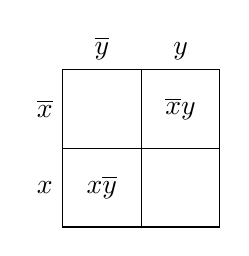
\begin{tikzpicture}
\pgfmathsetmacro{\kxstep}{1}
\pgfmathsetmacro{\kystep}{1}
\pgfmathsetmacro{\kpin}{0.75}
\pgfmathsetmacro{\kmv}{0.15}
\pgfmathsetmacro{\kmva}{0.1}
\draw[xstep=\kxstep,ystep=\kystep](0,0) grid (2*\kxstep,-2*\kystep);
%\draw(0,0)--++(135:\kpin)node[pos=0.75,above right]{$yz$}node[pos=0.75,below left]{$x$};
\foreach \kx/\xlb in {0/{\overline{y}},1/{y}}{\draw(\kx*\kxstep+\kxstep/2,0)node[above]{$\xlb$};}
\foreach \ky/\ylb in {0/{\overline{x}},1/{x}}{\draw(0,-\ky*\kystep-\kystep/2)node[left]{$\ylb$};}
\foreach \kx/\xlb in {1/{\overline{x}y}}{\draw(\kx*\kxstep+\kxstep/2,-\kystep/2)node[]{$\xlb$};}
\foreach \kx/\xlb in {0/{x\overline{y}}}{\draw(\kx*\kxstep+\kxstep/2,-1.5*\kystep)node[]{$\xlb$};}
%\draw[gray,dashed] ($(0,0)+(\kmv,-\kmv)$) rectangle ($(2*\kxstep,-2*\kystep)+(-\kmv,\kmv)$);
\end{tikzpicture}
\end{subfigure}\hfill
\begin{subfigure}{0.30\textwidth}
\centering
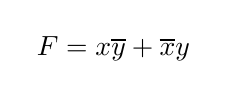
\begin{tikzpicture}
%\draw[step=1,thick](-2,-2) grid (2,1);
%\draw[step=0.1,gray](-2,-2) grid (2,1);
\draw(0,0) node[]{$F=x\overline{y}+\overline{x}y$};
\end{tikzpicture}
\end{subfigure}
\caption{قریبی خانے نہیں پائے جاتے۔}
\label{شکل_کارناف_قریبی_پانچ_مزید}
\end{figure}



\ابتدا{مشق}
ارکان ضرب کے مجموعہ کی سادہ صورت بوولین قوانین سے حاصل کر کے ثابت کریں کہ شکل \حوالہ{شکل_کارناف_قریبی_چوتھا_مزید} میں تفاعل کی سادہ مساوات \عددی{F=1} ہے۔
\انتہا{مشق}
\ابتدا{مشق}
 رکن ضرب نہ ہونے کی صورت میں ثابت کریں کہ تفاعل کی مساوات \عددی{F=0} ہو گی۔
\انتہا{مشق}

شکل \حوالہ{شکل_کارناف_قریبی_پانچ_مزید} میں ایسا تفاعل دیا گیا ہے جس کے خانے کسی مربع یا مستطیل میں نہیں گھیرے جا سکتے۔ایسے تفاعل کی مساوات کو سادہ نہیں بنایا جا سکتا۔


\جزوحصہ{تین متغیر تفاعل}
تین متغیر تفاعل اور اس کا کارناف نقشہ شکل \حوالہ{شکل_کارناف_قریبی_تین_متغیر} میں دکھایا گیا ہے۔کارناف نقشے میں دو قریبی خانوں کو گھیرنے والے تین مستطیل بنائے گئے ہیں۔ یاد رہے، مستطیل یوں بنانا لازمی ہے کہ اس میں \عددی{2^n} خانے سموئے جائیں، جہاں \عددی{n} عدد صحیح ہے۔ یوں تین خانوں کو گھیرنے کی اجازت نہیں۔
\begin{figure}
\centering
\begin{subfigure}{0.45\textwidth}
\centering
\begin{tikzpicture}
\pgfmathsetmacro{\kxstep}{1}
\pgfmathsetmacro{\kystep}{1}
\pgfmathsetmacro{\kpin}{0.75}
\pgfmathsetmacro{\kmv}{0.15}
\pgfmathsetmacro{\kmva}{0.10}
\draw[xstep=\kxstep,ystep=\kystep](0,0) grid (4*\kxstep,-2*\kystep);
%\draw(0,0)--++(135:\kpin)node[pos=0.75,above right]{$y$}node[pos=0.75,below left]{$x$};
\foreach \kx/\xlb in {0/{\overline{y}\,\overline{z}},1/{\overline{y}z},2/{yz},3/{y\overline{z}}}{\draw(\kx*\kxstep+\kxstep/2,0)node[above]{$\xlb$};}
\foreach \ky/\ylb in {0/{\overline{x}},1/{x}}{\draw(0,-\ky*\kystep-\kystep/2)node[left]{$\ylb$};}
\foreach \kx/\xlb in {0/{0},1/{0},2/1,3/0}{\draw(\kx*\kxstep+\kxstep/2,-\kystep/2)node[]{$\xlb$};}
\foreach \kx/\xlb in {0/{0},1/{1},2/1,3/1}{\draw(\kx*\kxstep+\kxstep/2,-1.5*\kystep)node[]{$\xlb$};}
\draw[gray,dashed] ($(\kxstep,-\kystep)+(\kmv,-\kmv)$) rectangle ($(3*\kxstep,-2*\kystep)+(-\kmv,\kmv)$);
\draw[gray,dashed] ($(2*\kxstep,-\kystep)+(\kmva,\kmva)$) rectangle ($(4*\kxstep,-2*\kystep)+(\kmva,-\kmva)$);
\draw[gray,dashed] ($(2*\kxstep,0)+(-\kmv,-\kmv)$) rectangle ($(3*\kxstep,-2*\kystep)+(\kmv,-2*\kmv)$);
\draw(4*\kxstep,-2*\kystep)++(0.1,\kystep/3) to [out=0,in=-135]++(0.5,0.5)node[right]{$xy$};
\draw(2.5*\kxstep,-2*\kystep-2*\kmv) to [out=-90,in=180]++(0.5,-0.5)node[right]{$yz$};
\draw(\kxstep+\kmv,-1.5*\kystep) to [out=180,in=45]++(-1,-1.25)node[left]{$xz$};
\end{tikzpicture}
\end{subfigure}\hfill
\begin{subfigure}{0.45\textwidth}
\centering
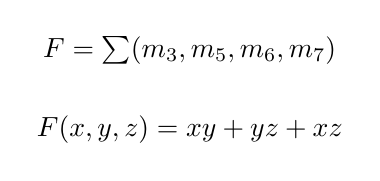
\begin{tikzpicture}
%\draw[step=1,thick](-2,-2) grid (2,1);
%\draw[step=0.1,gray](-2,-2) grid (2,1);
\draw(0,1)node[]{$F=\sum(m_3, m_5, m_6, m_7)$};
\draw(0,0) node[]{$F(x,y,z)=xy+yz+xz$};
\end{tikzpicture}
\end{subfigure}
\caption{تین متغیر تفاعل کے کارناف نقشے سے سادہ مساوات کا حصول۔}
\label{شکل_کارناف_قریبی_تین_متغیر}
\end{figure}


 درمیانی مستطیل \عددی{m_3} اور \عددی{m_7} گھیرتا ہے۔ ان خانوں کے ارکان ضرب میں \عددی{x} کی قیمت تبدیل ہوتی ہے، جبکہ \عددی{yz} دونوں میں مشترک ہے۔یوں ان کا سادہ رکن \عددی{yz} ہو گا۔باقی دو مستطیل سے \عددی{xy} اور \عددی{xz} حاصل ہو گا۔ یوں تفاعل کی سادہ مساوات ان کا مجموعہ \عددی{(F=xy+yz+xz)} ہو گا۔ اس مساوات کو ارکان ضرب کے مجموعہ سے بوولین قوانین کی مدد سے حاصل کر سکتے ہیں (جو آپ کو اگلی مشق میں کرنا ہو گا)۔
 \begin{gather}
 \begin{aligned}\label{مساوات_بوولین_تین_سادہ}
 F(x,y,z)&=\sum(m_3,m_5,m_6,m_7)\\
 &=\overline{x}yz+x\overline{y}z+xyz+xy\overline{z}& \text{\small\RL{(تفصیلی ارکان ضرب کا مجموعہ)}}&\\
 &=xy+yz+xz&\text{\small\RL{(سادہ ارکان ضرب کا مجموعہ)}}&
 \end{aligned}
 \end{gather}
اس مساوات کی دوسری لکیر میں، ارکان ضرب تمام آزاد متغیرات پر مشتمل ہیں۔اس طرح کے رکن ضرب کو تفصیلی رکن ضرب کہتے ہیں۔مساوات کی تیسری لکیر کے ارکان ضرب میں، آزاد متغیرات کی تعداد کم ہے۔ اس طرح کے رکن ضرب کو سادہ رکن ضرب کہتے ہیں۔اس کتاب میں، عموماً، دونوں اقسام رکن ضرب پکارے جائیں گے۔امید کی جاتی ہے، متن سے مطلوبہ مطلب واضح ہو گا؛جہاں ایسا نہ ہو، وہاں انہیں مکمل نام سے پکارا جائے گا۔ 





\ابتدا{مشق}
بوولین الجبرا استعمال کر کے مساوات \حوالہ{مساوات_بوولین_تین_سادہ} کی دوسری لکیر سے تیسری لکیر حاصل کریں۔ ساتھ ہی تسلی کر لیں کہ آپ شکل \حوالہ{شکل_کارناف_قریبی_تین_متغیر} کے کارناف نقشے سے سادہ ارکان ضرب حاصل کرنا جانتے ہیں۔
\انتہا{مشق}



شکل \حوالہ{شکل_کارناف_کی_تین_متغیر} میں تین متغیر کارناف نقشہ پیش کیا گیا ہے۔ نقشے میں \عددی{m_0=\overline{x}\,\overline{y}\,\overline{z}} اور
 \عددی{m_2=\overline{x}y\overline{z}} کا مجموعہ حاصل کرتے ہیں۔
 \begin{align*}
 m_0+m_2&=\overline{x}\,\overline{y}\,\overline{z}+\overline{x}y\overline{z}\\
 &=\overline{x}\,\overline{z}(\overline{y}+y)\\
 &=\overline{x}\,\overline{z}
 \end{align*}


\begin{figure}
\centering
\begin{subfigure}{0.50\textwidth}
\centering
\begin{tikzpicture}
\pgfmathsetmacro{\kxstep}{1}
\pgfmathsetmacro{\kystep}{1}
\pgfmathsetmacro{\kpin}{0.75}
\pgfmathsetmacro{\kmv}{0.15}
\pgfmathsetmacro{\kmva}{0.10}
\draw[xstep=\kxstep,ystep=\kystep](0,0) grid (4*\kxstep,-2*\kystep);
%\draw(0,0)--++(135:\kpin)node[pos=0.75,above right]{$y$}node[pos=0.75,below left]{$x$};
\foreach \kx/\xlb in {0/{\overline{y}\,\overline{z}},1/{\overline{y}z},2/{yz},3/{y\overline{z}}}{\draw(\kx*\kxstep+\kxstep/2,0)node[above]{$\xlb$};}
\foreach \ky/\ylb in {0/{\overline{x}},1/{x}}{\draw(0,-\ky*\kystep-\kystep/2)node[left]{$\ylb$};}
\foreach \kx/\xlb in {0/{1},1/{0},2/0,3/1}{\draw(\kx*\kxstep+\kxstep/2,-\kystep/2)node[]{$\xlb$};}
\foreach \kx/\xlb in {0/{0},1/{1},2/1,3/0}{\draw(\kx*\kxstep+\kxstep/2,-1.5*\kystep)node[]{$\xlb$};}
\draw[gray,dashed] ($(\kxstep,-\kystep)+(\kmv,-\kmv)$) rectangle ($(3*\kxstep,-2*\kystep)+(-\kmv,\kmv)$);
%\draw[gray,dashed] ($(2*\kxstep,-\kystep)+(\kmva,\kmva)$) rectangle ($(4*\kxstep,-2*\kystep)+(\kmva,-\kmva)$);
%\draw[gray,dashed] ($(2*\kxstep,0)+(-\kmv,-\kmv)$) rectangle ($(3*\kxstep,-2*\kystep)+(\kmv,-2*\kmv)$);
%\draw(4*\kxstep,-2*\kystep)++(0.1,\kystep/3) to [out=0,in=-135]++(0.5,0.5)node[right]{$xy$};
%\draw(2.5*\kxstep,-2*\kystep-2*\kmv) to [out=-90,in=180]++(0.5,-0.5)node[right]{$yz$};
\draw(\kxstep+\kmv,-1.5*\kystep) to [out=180,in=45]++(-1,-1.25)node[left]{$xz$};
\draw[gray,dashed] ($(0*\kxstep,0)+(-\kmv,-\kmv)$) --++ (1*\kxstep,0*\kystep)--++(0,-\kystep+2*\kmv)--++(-\kxstep,0);
\draw[gray,dashed] ($(4*\kxstep,0)+(\kmv,-\kmv)$) --++ (-1*\kxstep,0*\kystep)--++(0,-\kystep+2*\kmv)--++(\kxstep,0)coordinate(kend);
\draw(kend)++(0.05,0)--++(0.5,-0.5)node[right]{$\overline{x}\,\overline{z}$};
\end{tikzpicture}
\end{subfigure}\hfill
\begin{subfigure}{0.40\textwidth}
\centering
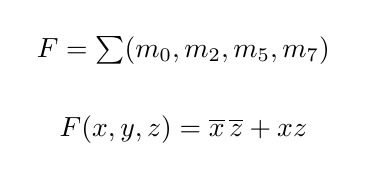
\begin{tikzpicture}
%\draw[step=1,thick](-2,-2) grid (2,1);
%\draw[step=0.1,gray](-2,-2) grid (2,1);
\draw(0,1)node[]{$F=\sum(m_0, m_2, m_5, m_7)$};
\draw(0,0) node[]{$F(x,y,z)=\overline{x}\,\overline{z}+xz$};
\end{tikzpicture}
\end{subfigure}
\caption{کارناف نقشے کے اطراف آپس میں ملائیں۔}
\label{شکل_کارناف_کی_تین_متغیر}
\end{figure}

ان تین متغیر ارکان ضرب کے مجموعے سے دو متغیر رکن ضرب حاصل ہوا۔یوں \عددی{m_0} اور \عددی{m_2} خانوں کو قریبی خانے تصور کرنا ہو گا۔ آئیں اس پر تفصیل سے گفتگو کریں۔

کارناف نقشے کے بایاں اور دایاں قطار کے خانوں کو قریبی تصور کریں۔ تصور میں اس کاغذ کو، جس پر کارناف نقشہ بنا ہو، یوں گول کریں کہ کاغذ کا بایاں اور دایاں کنارہ آپس مل جائیں۔ اب پہلی اور آخری قطار کے خانے قریبی ہوں گے۔ اسی طرح، دو سے زیادہ صفوں کی صورت میں، نچلی اور بالائی صف کے خانے قریبی ہوں گے۔ تصور میں کاغذ کو یوں لپیٹیں کہ اس کا نچلا کنارہ بالائی کنارے سے جا ملے۔ یوں ان صفوں کے خانوں کو قریبی تصور کیا جا سکتا ہے۔ 
	
شکل \حوالہ{شکل_کارناف_کی_تین_متغیر} میں \عددی{m_0} اور \عددی{m_2} کو مستطیل میں گھیرا دکھایا گیا ہے۔ (تصور کریں کہ لپیٹے گئے کاغذ پر ان خانوں کو مستطیل میں گھیرنے کے بعد، کاغذ کو دوبارہ سیدھا کیا گیا ہے؛ یوں مستطیل دو ٹکڑوں میں نظر آئے گا۔) ان خانوں میں \عددی{\overline{x}\,\overline{z}} مشترک ہے، جو ہمارے توقع کے عین مطابق ہے۔ خانہ \عددی{m_5} اور \عددی{m_7} میں \عددی{xz} مشترک ہے۔ یوں تفاعل کی سادہ مساوات ان سادہ ارکان کا مجموعہ \عددی{F=\overline{x}\,\overline{z}+xz} ہو گا۔


شکل \حوالہ{شکل_کارناف_چار_قریبی} میں تین متغیر کارناف نقشہ دیا گیا ہے، جس میں چار قریبی خانوں کے دو مربعے بنائے گئے ہیں۔آپ کارناف نقشے کو دیکھ کر تفاعل کی سادہ مساوات لکھ سکتے ہیں۔ (اگر آپ ایسا نہیں کر سکتے، تیار ہو جائیں! اگلی مشق میں یہی کہنے کو کہا گیا ہے۔)

\begin{figure}
\centering
\begin{subfigure}[t]{0.55\textwidth}
\centering
\begin{tikzpicture}
\pgfmathsetmacro{\kxstep}{1}
\pgfmathsetmacro{\kystep}{1}
\pgfmathsetmacro{\kpin}{0.75}
\pgfmathsetmacro{\kmv}{0.1}
\pgfmathsetmacro{\kmva}{0.20}
\draw[xstep=\kxstep,ystep=\kystep](0,0) grid (4*\kxstep,-2*\kystep);
%\draw(0,0)--++(135:\kpin)node[pos=0.75,above right]{$y$}node[pos=0.75,below left]{$x$};
\foreach \kx/\xlb in {0/{\overline{y}\,\overline{z}},1/{\overline{y}z},2/{yz},3/{y\overline{z}}}{\draw(\kx*\kxstep+\kxstep/2,0)node[above]{$\xlb$};}
\foreach \ky/\ylb in {0/{\overline{x}},1/{x}}{\draw(0,-\ky*\kystep-\kystep/2)node[left]{$\ylb$};}
\foreach \kx/\xlb in {0/1,1/0,2/1,3/1}{\draw(\kx*\kxstep+\kxstep/2,-\kystep/2)node[]{$\xlb$};}
\foreach \kx/\xlb in {0/1,1/0,2/1,3/1}{\draw(\kx*\kxstep+\kxstep/2,-1.5*\kystep)node[]{$\xlb$};}
\draw[gray,dashed] ($(2*\kxstep,-0*\kystep)+(\kmva,-\kmva)$) rectangle ($(4*\kxstep,-2*\kystep)+(-\kmva,\kmva)$);
%\draw[gray,dashed] ($(2*\kxstep,-\kystep)+(\kmva,\kmva)$) rectangle ($(4*\kxstep,-2*\kystep)+(\kmva,-\kmva)$);
%\draw[gray,dashed] ($(2*\kxstep,0)+(-\kmv,-\kmv)$) rectangle ($(3*\kxstep,-2*\kystep)+(\kmv,-2*\kmv)$);
%\draw(4*\kxstep,-2*\kystep)++(0.1,\kystep/3) to [out=0,in=-135]++(0.5,0.5)node[right]{$xy$};
%\draw(2.5*\kxstep,-2*\kystep-2*\kmv) to [out=-90,in=180]++(0.5,-0.5)node[right]{$yz$};
\draw(2*\kxstep+\kmva,-1.5*\kystep) to [out=180,in=45]++(-1,-1)node[left]{$y$};
\draw[gray,dashed] ($(0*\kxstep,0)+(-\kmv,-\kmv)$) --++ (1*\kxstep,0*\kystep)--++(0,-2*\kystep+2*\kmv)--++(-\kxstep,0);
\draw[gray,dashed] ($(4*\kxstep,0)+(\kmv,-\kmv)$) --++ (-1*\kxstep,0*\kystep)--++(0,-2*\kystep+2*\kmv)--++(\kxstep,0)coordinate(kend);
\draw(kend)++(0.05,0)--++(0.5,-0.5)node[right]{$\overline{z}$};
\end{tikzpicture}
\end{subfigure}\hfill
\begin{subfigure}[t]{0.35\textwidth}
\centering
\begin{tikzpicture}
\pgfmathsetmacro{\ksepX}{0.7}
\pgfmathsetmacro{\ksepY}{0.5}
\pgfmathsetmacro{\kmv}{0.2}
\foreach \n/\lbl in {0/{\overline{x}},1/{\overline{y}},2/{\overline{z}}}\draw(\n*\ksepX,0*\ksepY)node[]{$\lbl$};
\foreach \n/\lbl in {0/x,1/{\overline{y}},2/{\overline{z}}}\draw(\n*\ksepX,-1*\ksepY)node[]{$\lbl$};
\foreach \n/\lbl in {0/{\overline{x}},1/y,2/{\overline{z}}}\draw(\n*\ksepX,-2*\ksepY)node[]{$\lbl$};
\foreach \n/\lbl in {0/x,1/y,2/{\overline{z}}}\draw(\n*\ksepX,-3*\ksepY)node[]{$\lbl$};
\draw[dashed](1.5*\ksepX,0.5*\ksepY) rectangle (2.5*\ksepX,-3.5*\ksepY);
\draw(1*\ksepX,1.5*\ksepY)node[rectangle,text width=1.5cm,align=center]{\RTL{چار کونے}};
\end{tikzpicture}
\end{subfigure}
\caption{چار قریبی خانے۔}
\label{شکل_کارناف_چار_قریبی}
\end{figure}

\ابتدا{مشق}
 شکل \حوالہ{شکل_کارناف_چار_قریبی} میں دئے تفاعل کی سادہ مساوات کارناف نقشے سے حاصل کریں۔اسی مساوات کو بوولین الجبرا کی مدد سے حاصل کریں۔شکل میں چار کونوں کا مشترک حصہ \عددی{(\overline{z})} دکھایا گیا ہے۔ 
\انتہا{مشق}


\جزوحصہ{چار متغیر تفاعل}
چار آزاد متغیر تفاعل کے سولہ ارکان ضرب ہوں گے۔اس کے کارناف نقشے میں قریبی خانوں کو پہچانے کی خاطر نقشے کو ایسی سطح پر بنا ہوا تصور کریں کہ نقشے کی دایاں قطار نقشے کی بائیں قطار سے جڑا ہو۔اسی طرح نقشے کی بالائی صف اور نچلی صف سے آپس میں جڑے ہوں۔یوں \عددی{m_4} خانہ \عددی{m_6} خانے سے جڑتا ہے، اور \عددی{m_1} خانہ \عددی{m_9} خانے سے جڑتا ہے۔

اس نقشے میں دو، چار، آٹھ اور سولہ قریبی خانے بنانا ممکن ہے۔دو قریبی خانوں کے ارکان ضرب کا مجموعہ ایک رکن ضرب دے گا، جس میں تین متغیرات ہوں گے۔چار قریبی خانوں کے ارکان ضرب کا مجموعہ ایک رکن ضرب دے گا، جس میں دو آزاد متغیرات ہوں گے۔آٹھ قریبی خانوں کے ارکان ضرب کا مجموعہ ایک رکن ضرب دے گا، جس میں ایک متغیر ہو گا، جبکہ سولہ قریبی خانوں کے ارکان ضرب کا مجموعہ \عددی{1} کے برابر ہو گا۔

چار متغیر کارناف نقشوں کی چند مثالیں دیکھتے ہیں۔

\ابتدا{مثال}\شناخت{مثال_بوولین_چار_پہلا}
 درج ذیل تفاعل کی سادہ مساوات شکل \حوالہ{شکل_کارناف_مثال_چار_پہلا_متغیر} میں پیش کی گئی ہے۔	
\begin{align*}
F(w,x,y,z)=\sum(m_0, m_2,m_4,m_6,m_8,m_{10}, m_{12},m_{13},m_{14}, m_{15})
\end{align*}
%
\begin{figure}
\centering
\begin{subfigure}{0.60\textwidth}
\centering
\begin{tikzpicture}
\pgfmathsetmacro{\kxstep}{1}
\pgfmathsetmacro{\kystep}{1}
\pgfmathsetmacro{\kpin}{0.75}
\pgfmathsetmacro{\kmv}{0.15}
\pgfmathsetmacro{\kmva}{0.10}
\draw[xstep=\kxstep,ystep=\kystep](0,0) grid (4*\kxstep,-4*\kystep);
%\draw(0,0)--++(135:\kpin)node[pos=0.75,above right]{$y$}node[pos=0.75,below left]{$x$};
\foreach \kx/\xlb in {0/{\overline{y}\,\overline{z}},1/{\overline{y}z},2/{yz},3/{y\overline{z}}}{\draw(\kx*\kxstep+\kxstep/2,0)node[above]{$\xlb$};}
\foreach \ky/\ylb in {0/{\overline{w}\,\overline{x}},1/{\overline{w}x},2/{wx},3/{w\overline{x}}}{\draw(0,-\ky*\kystep-\kystep/2)node[left]{$\ylb$};}
\foreach \kx/\xlb in {0/{1},3/1}{\draw(\kx*\kxstep+\kxstep/2,-\kystep/2)node[]{$\xlb$};}
\foreach \kx/\xlb in {0/{1},3/1}{\draw(\kx*\kxstep+\kxstep/2,-1.5*\kystep)node[]{$\xlb$};}
\foreach \kx/\xlb in {0/{1},1/1,2/1,3/1}{\draw(\kx*\kxstep+\kxstep/2,-2.5*\kystep)node[]{$\xlb$};}
\foreach \kx/\xlb in {0/{1},3/1}{\draw(\kx*\kxstep+\kxstep/2,-3.5*\kystep)node[]{$\xlb$};}
\draw[gray,dashed] ($(0,-2*\kystep)+(\kmv,-\kmv)$) rectangle ($(4*\kxstep,-3*\kystep)+(-\kmv,\kmv)$);
%\draw[gray,dashed] ($(2*\kxstep,-\kystep)+(\kmva,\kmva)$) rectangle ($(4*\kxstep,-2*\kystep)+(\kmva,-\kmva)$);
%\draw[gray,dashed] ($(2*\kxstep,0)+(-\kmv,-\kmv)$) rectangle ($(3*\kxstep,-2*\kystep)+(\kmv,-2*\kmv)$);
%\draw(4*\kxstep,-2*\kystep)++(0.1,\kystep/3) to [out=0,in=-135]++(0.5,0.5)node[right]{$xy$};
%\draw(2.5*\kxstep,-2*\kystep-2*\kmv) to [out=-90,in=180]++(0.5,-0.5)node[right]{$yz$};
\draw($(4*\kxstep,-2.5*\kystep)+(-\kmv,0)$) to [out=0,in=180]++(0.5,0.5)node[right]{$wx$};
\draw[gray,dashed] ($(0*\kxstep,0)+(-\kmv,-\kmv)$) --++ (1*\kxstep,0*\kystep)--++(0,-4*\kystep+2*\kmv)--++(-\kxstep,0);
\draw[gray,dashed] ($(4*\kxstep,0)+(\kmv,-\kmv)$) --++ (-1*\kxstep,0*\kystep)--++(0,-4*\kystep+2*\kmv)--++(\kxstep+2*\kmv,0)coordinate(kend);
\draw(kend)++(-0.05,0)--++(0.5,-0.5)node[right]{$\overline{z}$};
\end{tikzpicture}
\end{subfigure}\hfill
\begin{subfigure}{0.30\textwidth}
\centering
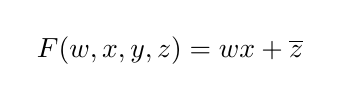
\begin{tikzpicture}
%\draw[step=1,thick](-2,-2) grid (2,1);
%\draw[step=0.1,gray](-2,-2) grid (2,1);
%\draw(0,1)node[]{$F=\sum(m_0, m_2, m_5, m_7)$};
\draw(0,0) node[]{$F(w,x,y,z)=wx+\overline{z}$};
\end{tikzpicture}
\end{subfigure}
\caption{چار متغیر نقشہ ( برائے مثال \حوالہ{مثال_بوولین_چار_پہلا})}
\label{شکل_کارناف_مثال_چار_پہلا_متغیر}
\end{figure}
\انتہا{مثال}
\ابتدا{مثال}\شناخت{مثال_بوولین_چار_دوسرا}
 درج ذیل تفاعلات کی سادہ مساوات حاصل کریں۔
\begin{align*}
F(w,x,y,z)&=\sum(m_0,m_5,m_7,m_{10},m_{11},m_{13},m_{15})\\
F(w,x,y,z)&=\sum(m_0,m_2,m_8,m_{10})
\end{align*}
%
\begin{figure}
\centering
\begin{subfigure}{0.45\textwidth}
\centering
\begin{tikzpicture}
\pgfmathsetmacro{\kxstep}{1}
\pgfmathsetmacro{\kystep}{1}
\pgfmathsetmacro{\kpin}{0.75}
\pgfmathsetmacro{\kmv}{0.15}
\pgfmathsetmacro{\kmva}{0.10}
\draw[xstep=\kxstep,ystep=\kystep](0,0) grid (4*\kxstep,-4*\kystep);
%\draw(0,0)--++(135:\kpin)node[pos=0.75,above right]{$y$}node[pos=0.75,below left]{$x$};
\foreach \kx/\xlb in {0/{\overline{y}\,\overline{z}},1/{\overline{y}z},2/{yz},3/{y\overline{z}}}{\draw(\kx*\kxstep+\kxstep/2,0)node[above]{$\xlb$};}
\foreach \ky/\ylb in {0/{\overline{w}\,\overline{x}},1/{\overline{w}x},2/{wx},3/{w\overline{x}}}{\draw(0,-\ky*\kystep-\kystep/2)node[left]{$\ylb$};}
\foreach \kx/\xlb in {0/{1}}{\draw(\kx*\kxstep+\kxstep/2,-\kystep/2)node[]{$\xlb$};}
\foreach \kx/\xlb in {1/{1},2/1}{\draw(\kx*\kxstep+\kxstep/2,-1.5*\kystep)node[]{$\xlb$};}
\foreach \kx/\xlb in {1/{1},2/1}{\draw(\kx*\kxstep+\kxstep/2,-2.5*\kystep)node[]{$\xlb$};}
\foreach \kx/\xlb in {2/1,3/1}{\draw(\kx*\kxstep+\kxstep/2,-3.5*\kystep)node[]{$\xlb$};}
\draw[gray,dashed] ($(1*\kxstep,-1*\kystep)+(\kmv,-\kmv)$) rectangle ($(3*\kxstep,-3*\kystep)+(-\kmv,\kmv)$);
\draw[gray,dashed] ($(2*\kxstep,-3*\kystep)+(\kmv,-\kmv)$) rectangle ($(4*\kxstep,-4*\kystep)+(-\kmv,\kmv)$);
\draw(4*\kxstep-\kmv,-3.5*\kystep) to [out=0,in=180]++(0.5,0.5)node[right]{$w\overline{x}x$};
\draw(3*\kxstep-\kmv,-1.5*\kystep) to [out=0,in=180]++(1.52,0.4)node[right]{$xz$};
\draw(0.25*\kxstep,-0.25*\kystep) to [out=180,in=0]++(-0.5,0.25)node[left]{$\overline{w}\,\overline{x}\,\overline{y}\,\overline{z}x$};
\path(0,-4*\kystep)--++(0,-0.5); %gives space between the map and its equation in the next tikzpic
\end{tikzpicture}
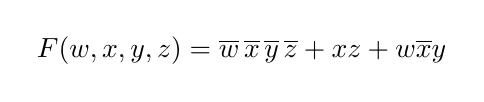
\begin{tikzpicture}
\draw(0,0)node[]{$F(w,x,y,z)=\overline{w}\,\overline{x}\,\overline{y}\,\overline{z}+xz+w\overline{x}y$};
\end{tikzpicture}
\caption{}
\end{subfigure}\hfill
\begin{subfigure}{0.45\textwidth}
\centering
\begin{tikzpicture}
\pgfmathsetmacro{\kxstep}{1}
\pgfmathsetmacro{\kystep}{1}
\pgfmathsetmacro{\kpin}{0.75}
\pgfmathsetmacro{\kmv}{0.15}
\pgfmathsetmacro{\kmva}{0.10}
\draw[xstep=\kxstep,ystep=\kystep](0,0) grid (4*\kxstep,-4*\kystep);
%\draw(0,0)--++(135:\kpin)node[pos=0.75,above right]{$y$}node[pos=0.75,below left]{$x$};
\foreach \kx/\xlb in {0/{\overline{y}\,\overline{z}},1/{\overline{y}z},2/{yz},3/{y\overline{z}}}{\draw(\kx*\kxstep+\kxstep/2,0)node[above]{$\xlb$};}
\foreach \ky/\ylb in {0/{\overline{w}\,\overline{x}},1/{\overline{w}x},2/{wx},3/{w\overline{x}}}{\draw(0,-\ky*\kystep-\kystep/2)node[left]{$\ylb$};}
\foreach \kx/\xlb in {0/{1},3/1}{\draw(\kx*\kxstep+\kxstep/2,-\kystep/2)node[]{$\xlb$};}
%\foreach \kx/\xlb in {1/{1},2/1}{\draw(\kx*\kxstep+\kxstep/2,-1.5*\kystep)node[]{$\xlb$};}
%\foreach \kx/\xlb in {1/{1},2/1}{\draw(\kx*\kxstep+\kxstep/2,-2.5*\kystep)node[]{$\xlb$};}
\foreach \kx/\xlb in {0/1,3/1}{\draw(\kx*\kxstep+\kxstep/2,-3.5*\kystep)node[]{$\xlb$};}
%\draw[gray,dashed] ($(1*\kxstep,-1*\kystep)+(\kmv,-\kmv)$) rectangle ($(3*\kxstep,-3*\kystep)+(-\kmv,\kmv)$);
%\draw[gray,dashed] ($(2*\kxstep,-3*\kystep)+(\kmv,-\kmv)$) rectangle ($(4*\kxstep,-4*\kystep)+(-\kmv,\kmv)$);
\draw[gray,dashed] ($(0,-1*\kystep)+(-\kmv,\kmv)$)--++(1*\kxstep,0)--++(0,\kystep+\kmv);
\draw[gray,dashed] ($(0,-3*\kystep)+(-\kmv,-\kmv)$)--++(1*\kxstep,0)--++(0,-\kystep-\kmv);
\draw[gray,dashed] ($(3*\kxstep,-0*\kystep)+(\kmv,\kmv)$)--++(0,-1*\kystep)--++(\kxstep+\kmv,0);
\draw[gray,dashed] ($(3*\kxstep,-4*\kystep)+(\kmv,-\kmv)$)--++(0,1*\kystep)--++(\kxstep+\kmv,0);
\path(0,-4*\kystep)--++(0,-0.5); %gives space between the map and its equation in the next tikzpic
\end{tikzpicture}
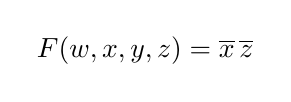
\begin{tikzpicture}
\draw(0,0)node[]{$F(w,x,y,z)=\overline{x}\,\overline{z}$};
\end{tikzpicture}
\caption{}
\end{subfigure}
\caption{چار متغیر نقشہ ( برائے مثال \حوالہ{مثال_بوولین_چار_دوسرا})}
\label{شکل_کارناف_مثال_چار_دوسرا_متغیر}
\end{figure}

\ترچھا{حل:}\quad
پہلا تفاعل شکل \حوالہ{شکل_کارناف_مثال_چار_دوسرا_متغیر}-الف میں دکھایا گیا ہے، جہاں چار قریبی خانے سادہ رکن ضرب \عددی{(xz)}، جبکہ دو قریبی خانے \عددی{w\overline{x}y} رکن ضرب دیں گے، اور ایک خانہ جو کسی کے قریب نہیں پایا جاتا رکن \عددی{\overline{w}\,\overline{x}\,\overline{y}\,\overline{z}} دے گا۔یوں تفاعل کی سادہ مساوات ان ارکان کا مجموعہ \عددی{F=\overline{w}\,\overline{x}\,\overline{y}\,\overline{z}+xz+w\overline{x}y} ہو گا۔


دوسرا تفاعل شکل \حوالہ{شکل_کارناف_مثال_چار_دوسرا_متغیر}-ب میں پیش کیا گیا ہے، جہاں چار کونوں کو قریبی تصور کریں، جو رکن \عددی{\overline{x}\,\overline{z}} دیں 
گے۔یہی اس تفاعل کی سادہ مساوات \عددی{F=\overline{x}\,\overline{z}} ہے۔
\انتہا{مثال}
\ابتدا{مشق}
شکل \حوالہ{شکل_کارناف_مثال_چار_دوسرا_متغیر}-ب کے چار خانوں کے ارکان ضرب کے مجموعہ کا سادہ روپ، بوولین قوانین کی مدد سے حاصل کر کے ثابت کریں کہ یہ قریبی خانے ہیں۔
\انتہا{مشق}
\ابتدا{مثال}\شناخت{مثال_بوولین_تین_بلاشرکت}
تین آزاد متغیرات کے بلا شرکت گیٹ کا کارناف نقشہ حاصل کریں۔

\begin{figure}
\centering
\begin{subfigure}{0.45\textwidth}
\centering
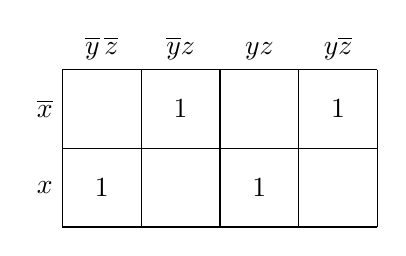
\begin{tikzpicture}
\pgfmathsetmacro{\kxstep}{1}
\pgfmathsetmacro{\kystep}{1}
\pgfmathsetmacro{\kpin}{0.75}
\pgfmathsetmacro{\kmv}{0.15}
\pgfmathsetmacro{\kmva}{0.10}
\draw[xstep=\kxstep,ystep=\kystep](0,0) grid (4*\kxstep,-2*\kystep);
%\draw(0,0)--++(135:\kpin)node[pos=0.75,above right]{$y$}node[pos=0.75,below left]{$x$};
\foreach \kx/\xlb in {0/{\overline{y}\,\overline{z}},1/{\overline{y}z},2/{yz},3/{y\overline{z}}}{\draw(\kx*\kxstep+\kxstep/2,0)node[above]{$\xlb$};}
\foreach \ky/\ylb in {0/{\overline{x}},1/x}{\draw(0,-\ky*\kystep-\kystep/2)node[left]{$\ylb$};}
\foreach \kx/\xlb in {1/{1},3/1}{\draw(\kx*\kxstep+\kxstep/2,-\kystep/2)node[]{$\xlb$};}
\foreach \kx/\xlb in {0/{1},2/1}{\draw(\kx*\kxstep+\kxstep/2,-1.5*\kystep)node[]{$\xlb$};}
%\foreach \kx/\xlb in {1/{1},2/1}{\draw(\kx*\kxstep+\kxstep/2,-2.5*\kystep)node[]{$\xlb$};}
%\foreach \kx/\xlb in {0/1,3/1}{\draw(\kx*\kxstep+\kxstep/2,-3.5*\kystep)node[]{$\xlb$};}
%\draw[gray,dashed] ($(1*\kxstep,-1*\kystep)+(\kmv,-\kmv)$) rectangle ($(3*\kxstep,-3*\kystep)+(-\kmv,\kmv)$);
%\draw[gray,dashed] ($(2*\kxstep,-3*\kystep)+(\kmv,-\kmv)$) rectangle ($(4*\kxstep,-4*\kystep)+(-\kmv,\kmv)$);
%\draw[gray,dashed] ($(0,-1*\kystep)+(-\kmv,\kmv)$)--++(1*\kxstep,0)--++(0,\kystep+\kmv);
%\draw[gray,dashed] ($(0,-3*\kystep)+(-\kmv,-\kmv)$)--++(1*\kxstep,0)--++(0,-\kystep-\kmv);
\end{tikzpicture}
\end{subfigure}\hfill
\begin{subfigure}{0.45\textwidth}
\centering
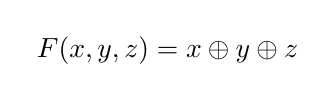
\begin{tikzpicture}
\draw(0,0)node[]{$F(x,y,z)=x\oplus y \oplus z$};
\end{tikzpicture}
\end{subfigure}
\caption{تین متغیر بلا شرکت گیٹ کا نقشہ (برائے مثال \حوالہ{مثال_بوولین_تین_بلاشرکت})}
\label{شکل_بوولین_تین_بلاشرکت}
\end{figure}
\ترچھا{حل:}\quad
شکل \حوالہ{شکل_بوولین_تین_بلاشرکت} میں نقشہ پیش ہے۔اس میں قریب خانے نہیں پائے جاتے، لہٰذا اس کی مساوات مزید سادہ نہیں بنائی جا سکتی۔ 
\انتہا{مثال}


\جزوحصہ{سادہ مساوات سے تفاعل کے ارکان ضرب کا حصول}
کسی بھی تفاعل کی سادہ مساوات کا حصول بذریعہ کارناف نقشہ آپ نے دیکھا۔اس حصے میں اس طریقہ کار کو اُلٹ چلا کر تفاعل کی سادہ مساوات سے ارکان ضرب کا مجموعہ حاصل کیا جائے گا۔یہ ترکیب مثال سے بہتر سمجھ آئی گی۔

\ابتدا{مثال}\شناخت{مثال_بوولین_الٹ_رخ}
درج ذیل سادہ مساوات سے تفاعل کے ارکان ضرب کا مجموعہ دریافت کریں۔
\begin{align*}
F(x,y,z)=y+\overline{x}\,\overline{z}
\end{align*}
\ترچھا{حل:}\quad
شکل \حوالہ{شکل_بوولین_الٹ_رخ} میں سادہ مساوات سے کارناف نقشہ حاصل کیا گیا، جس سے مجموعہ ارکان ضرب لکھا گیا ۔
\begin{figure}
\centering
\begin{subfigure}{0.45\textwidth}
\centering
\begin{tikzpicture}
\pgfmathsetmacro{\kxstep}{1}
\pgfmathsetmacro{\kystep}{1}
\pgfmathsetmacro{\kpin}{0.75}
\pgfmathsetmacro{\kmv}{0.1}
\pgfmathsetmacro{\kmva}{0.20}
\draw[xstep=\kxstep,ystep=\kystep](0,0) grid (4*\kxstep,-2*\kystep);
%\draw(0,0)--++(135:\kpin)node[pos=0.75,above right]{$y$}node[pos=0.75,below left]{$x$};
\foreach \kx/\xlb in {0/{\overline{y}\,\overline{z}},1/{\overline{y}z},2/{yz},3/{y\overline{z}}}{\draw(\kx*\kxstep+\kxstep/2,0)node[above]{$\xlb$};}
\foreach \ky/\ylb in {0/{\overline{x}},1/x}{\draw(0,-\ky*\kystep-\kystep/2)node[left]{$\ylb$};}
\foreach \kx/\xlb in {0/{1},2/1,3/1}{\draw(\kx*\kxstep+\kxstep/2,-\kystep/2)node[]{$\xlb$};}
\foreach \kx/\xlb in {2/{1},3/1}{\draw(\kx*\kxstep+\kxstep/2,-1.5*\kystep)node[]{$\xlb$};}
%\foreach \kx/\xlb in {1/{1},2/1}{\draw(\kx*\kxstep+\kxstep/2,-2.5*\kystep)node[]{$\xlb$};}
%\foreach \kx/\xlb in {0/1,3/1}{\draw(\kx*\kxstep+\kxstep/2,-3.5*\kystep)node[]{$\xlb$};}
\draw[gray,dashed] ($(2*\kxstep,-0*\kystep)+(\kmv,-\kmv)$) rectangle ($(4*\kxstep,-2*\kystep)+(-\kmv,\kmv)$);
\draw[gray,dashed] ($(0*\kxstep,-0*\kystep)+(-\kmva,-\kmva)$)--++(\kxstep,0)--++(0,-\kystep+2*\kmva)--++(-\kxstep,0);
\draw[gray,dashed] ($(4*\kxstep,-0*\kystep)+(\kmva,-\kmva)$)--++(-\kxstep,0)--++(0,-\kystep+2*\kmva)
--++(\kxstep,0)coordinate(kend);
%\draw[gray,dashed] ($(0,-1*\kystep)+(-\kmv,\kmv)$)--++(1*\kxstep,0)--++(0,\kystep+\kmv);
%\draw[gray,dashed] ($(0,-3*\kystep)+(-\kmv,-\kmv)$)--++(1*\kxstep,0)--++(0,-\kystep-\kmv);
\draw[](4*\kxstep-\kmv,-1.5*\kystep) to [out=0,in=180]++(0.5,-0.25)node[right]{$y$};
\draw[](kend) to [out=0,in=180]++(0.5,0.25)node[right]{$\overline{x}\,\overline{z}$};
\end{tikzpicture}
\end{subfigure}\hfill
\begin{subfigure}{0.45\textwidth}
\centering
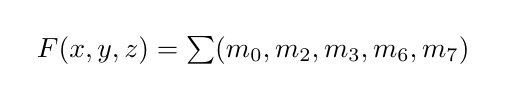
\begin{tikzpicture}
\draw(0,0)node[]{$F(x,y,z)=\sum (m_0,m_2,m_3,m_6,m_7)$};
\end{tikzpicture}
\end{subfigure}
\caption{سادہ مساوات سے ارکان ضرب کے مجموعہ کا حصول (مثال \حوالہ{مثال_بوولین_الٹ_رخ})۔}
\label{شکل_بوولین_الٹ_رخ}
\end{figure}
\انتہا{مثال}


\حصہ{ ضرب بعد از جمع  روپ  میں سادہ مساوات}
 کارناف نقشے کے ان خانوں میں \عددی{1} پُر کیا جاتا ہے جن میں تفاعل کے بوولین جدول میں ارکان ضرب کی قیمت \عددی{1} ہو۔تفاعل کے متمم کے بوولین جدول میں جہاں پہلے \عددی{0} تھا اب وہاں \عددی{1} ہو گا۔ اس جدول کے کارناف نقشے سے ارکان ضرب کے مجموعے کی مساوات، تفاعل کے متمم کی سادہ مساوات ہو گی۔یہ مساوات مجموعہ ارکان ضرب کے روپ میں ہو گی، جس کا متمم لے کر اصل تفاعل کی ( ضرب بعد از جمع  روپ میں) سادہ مساوات حاصل ہو گی۔ایک مثال سے اس بات کی وضاحت کرتے ہیں۔

\ابتدا{مثال}\شناخت{مثال_بوولین_متمم_حصول}
مندرجہ ذیل تفاعل کی  مجموعہ ارکان ضرب اور  ضرب بعد از جمع  شکل میں سادہ مساوات حاصل کریں۔
\begin{align*}
F(x,y,z)=\sum(m_2,m_3,m_4,m_5)
\end{align*}
\ترچھا{حل:}\quad
شکل \حوالہ{شکل_بوولین_متمم_سے_حصول}-الف میں تفاعل اور اس کے متمم کا جدول پیش کیا گیا ہے۔ ،شکل-ب میں تفاعل کی مساوات، ارکان ضرب کے مجموعہ کی صورت میں دی گئی ہے۔ شکل-ج میں دی گئی مساوات، تفاعل کے متمم کی ہے، جس کا متمم لے کر (اور بوولین کلیات استعمال کر کے) تفاعل کے ارکان جمع کی ضرب کی (درج ذیل) سادہ مساوات حاصل ہو گی۔
\begin{align*}
F=\overline{\overline{F}}&=\overline{\overline{x}\,\overline{y}+xy}\\
&=(\overline{\overline{x}\,\overline{y}})(\overline{xy})\\
&=(\overline{\overline{x}}+\overline{\overline{y}})(\overline{x}+\overline{y})\\
&=(x+y)(\overline{x}+\overline{y})
\end{align*}
%
\begin{figure}
\centering
\begin{subfigure}{0.45\textwidth}
\centering
\begin{otherlanguage}{english}
\begin{tabular}{CCC|CC}
\toprule
x&y&z&F&\overline{F}\\
\midrule
0&0&0&0&1\\
0&0&1&0&1\\
0&1&0&1&0\\
0&1&1&1&0\\
1&0&0&1&0\\
1&0&1&1&0\\
1&1&0&0&1\\
1&1&1&0&1\\
\bottomrule
\end{tabular}
\end{otherlanguage}
\caption{}
\end{subfigure}%
\begin{subfigure}{0.45\textwidth}
\centering
\begin{subfigure}{1\textwidth}
\centering
\begin{tikzpicture}
\pgfmathsetmacro{\kxstep}{1}
\pgfmathsetmacro{\kystep}{1}
\pgfmathsetmacro{\kpin}{0.75}
\pgfmathsetmacro{\kmv}{0.15}
\pgfmathsetmacro{\kmva}{0.10}
\draw[xstep=\kxstep,ystep=\kystep](0,0) grid (4*\kxstep,-2*\kystep);
%\draw(0,0)--++(135:\kpin)node[pos=0.75,above right]{$y$}node[pos=0.75,below left]{$x$};
\foreach \kx/\xlb in {0/{\overline{y}\,\overline{z}},1/{\overline{y}z},2/{yz},3/{y\overline{z}}}{\draw(\kx*\kxstep+\kxstep/2,0)node[above]{$\xlb$};}
\foreach \ky/\ylb in {0/{\overline{x}},1/{x}}{\draw(0,-\ky*\kystep-\kystep/2)node[left]{$\ylb$};}
\foreach \kx/\xlb in {0/{0},1/0,2/1,3/1}{\draw(\kx*\kxstep+\kxstep/2,-\kystep/2)node[]{$\xlb$};}
\foreach \kx/\xlb in {0/{1},1/1,2/0,3/0}{\draw(\kx*\kxstep+\kxstep/2,-1.5*\kystep)node[]{$\xlb$};}
%\foreach \kx/\xlb in {1/{1},2/1}{\draw(\kx*\kxstep+\kxstep/2,-2.5*\kystep)node[]{$\xlb$};}
%\foreach \kx/\xlb in {0/1,3/1}{\draw(\kx*\kxstep+\kxstep/2,-3.5*\kystep)node[]{$\xlb$};}
\draw[gray,dashed] ($(2*\kxstep,-0*\kystep)+(\kmv,-\kmv)$) rectangle ($(4*\kxstep,-1*\kystep)+(-\kmv,\kmv)$);
\draw[gray,dashed] ($(0*\kxstep,-1*\kystep)+(\kmv,-\kmv)$) rectangle ($(2*\kxstep,-2*\kystep)+(-\kmv,\kmv)$);
%\draw[gray,dashed] ($(0,-1*\kystep)+(-\kmv,\kmv)$)--++(1*\kxstep,0)--++(0,\kystep+\kmv);
%\draw[gray,dashed] ($(0,-3*\kystep)+(-\kmv,-\kmv)$)--++(1*\kxstep,0)--++(0,-\kystep-\kmv);
%\draw[gray,dashed] ($(3*\kxstep,-0*\kystep)+(\kmv,\kmv)$)--++(0,-1*\kystep)--++(\kxstep+\kmv,0);
%\draw[gray,dashed] ($(3*\kxstep,-4*\kystep)+(\kmv,-\kmv)$)--++(0,1*\kystep)--++(\kxstep+\kmv,0);
\draw(3*\kxstep,-2*\kystep-0.5)node[right]{\text{\RL{(ب)}}}node[left]{$F=\overline{x}y+x\overline{y}$};
\path(0,-3*\kystep)node[]{};
\end{tikzpicture}
\end{subfigure}
\begin{subfigure}{1\textwidth}
\centering
\begin{tikzpicture}
\pgfmathsetmacro{\kxstep}{1}
\pgfmathsetmacro{\kystep}{1}
\pgfmathsetmacro{\kpin}{0.75}
\pgfmathsetmacro{\kmv}{0.15}
\pgfmathsetmacro{\kmva}{0.10}
\draw[xstep=\kxstep,ystep=\kystep](0,0) grid (4*\kxstep,-2*\kystep);
%\draw(0,0)--++(135:\kpin)node[pos=0.75,above right]{$y$}node[pos=0.75,below left]{$x$};
\foreach \kx/\xlb in {0/{\overline{y}\,\overline{z}},1/{\overline{y}z},2/{yz},3/{y\overline{z}}}{\draw(\kx*\kxstep+\kxstep/2,0)node[above]{$\xlb$};}
\foreach \ky/\ylb in {0/{\overline{x}},1/{x}}{\draw(0,-\ky*\kystep-\kystep/2)node[left]{$\ylb$};}
\foreach \kx/\xlb in {0/{1},1/1,2/0,3/0}{\draw(\kx*\kxstep+\kxstep/2,-\kystep/2)node[]{$\xlb$};}
\foreach \kx/\xlb in {0/{0},1/0,2/1,3/1}{\draw(\kx*\kxstep+\kxstep/2,-1.5*\kystep)node[]{$\xlb$};}
%\foreach \kx/\xlb in {1/{1},2/1}{\draw(\kx*\kxstep+\kxstep/2,-2.5*\kystep)node[]{$\xlb$};}
%\foreach \kx/\xlb in {0/1,3/1}{\draw(\kx*\kxstep+\kxstep/2,-3.5*\kystep)node[]{$\xlb$};}
\draw[gray,dashed] ($(2*\kxstep,-1*\kystep)+(\kmv,-\kmv)$) rectangle ($(4*\kxstep,-2*\kystep)+(-\kmv,\kmv)$);
\draw[gray,dashed] ($(0*\kxstep,-0*\kystep)+(\kmv,-\kmv)$) rectangle ($(2*\kxstep,-1*\kystep)+(-\kmv,\kmv)$);
%\draw[gray,dashed] ($(0,-1*\kystep)+(-\kmv,\kmv)$)--++(1*\kxstep,0)--++(0,\kystep+\kmv);
%\draw[gray,dashed] ($(0,-3*\kystep)+(-\kmv,-\kmv)$)--++(1*\kxstep,0)--++(0,-\kystep-\kmv);
%\draw[gray,dashed] ($(3*\kxstep,-0*\kystep)+(\kmv,\kmv)$)--++(0,-1*\kystep)--++(\kxstep+\kmv,0);
%\draw[gray,dashed] ($(3*\kxstep,-4*\kystep)+(\kmv,-\kmv)$)--++(0,1*\kystep)--++(\kxstep+\kmv,0);
\draw(3*\kxstep,-2*\kystep-0.5)node[right]{\text{\RL{(ج)}}}node[left]{$\overline{F}=\overline{x}\,\overline{y}+x y$};
\end{tikzpicture}
\end{subfigure}
\end{subfigure}
\caption{مجموعہ ارکان ضرب اور  ضرب بعد از جمع کی شکل  میں سادہ مساوات (مثال \حوالہ{مثال_بوولین_متمم_حصول})۔}
\label{شکل_بوولین_متمم_سے_حصول}
\end{figure}
\انتہا{مثال}

\حصہ{غیر دلچسپ حال}
 ہم نے اب تک جتنے تفاعل دیکھے، ان میں مداخل کی تمام صورتوں کے مطابقتی مخارج دستیاب اور ضروری تھے۔بعض اوقات مداخل کی چند قیمتیں ممکن نہیں ہوں گی یا ان کے مطابقتی مخارج استعمال نہیں ہوں گے۔مداخل کے ان قیمتوں کو  \اصطلاح{غیر دلچسپ حال }\فرہنگ{غیر دلچسپ حال}\حاشیہب{don't care states}\فرہنگ{don't care} کہتے ہیں۔ 

تفاعل کی سادہ مساوات حاصل کرتے وقت، کارناف نقشے کے غیر دلچسپ حال خانوں میں \عددی{0} یا \عددی{1} کی بجائے \عددی{d} درج کیا جاتا ہے۔قریبی خانے گھیرتے وقت اگر کسی غیر ضروری خانے میں \عددی{1} تصور کرنے سے زیادہ سادہ مساوات حاصل ہو تو اس خانے میں \عددی{1} تصور کیا جاتا ہے، اور اگر اس میں \عددی{0} تصور کرنے سے زیادہ سادہ مساوات حاصل ہوتی ہے تو اس میں \عددی{0} تصور کیا جاتا ہے۔


\ابتدا{مثال}\شناخت{مثال_بوولین_غیر_دلچسپ_پہلا}
درج ذیل تفاعل کی سادہ مساوات، مجموعہ ارکان ضرب اور  ضرب بعد از جمع کے روپ میں حاصل کریں۔
\begin{align*}
F(x,y)&=\sum (m_0,m_3)\\
d(x,y)&=\sum (m_2)
\end{align*}
%
\begin{figure}
\centering
\begin{subfigure}{0.33\textwidth}
\centering
\begin{otherlanguage}{english}
\begin{tabular}{CC|CC}
\toprule
x&y&F&\overline{F}\\
\midrule
0&0&0&1\\
0&1&1&0\\
1&0&d&d\\
1&1&1&0\\
\bottomrule
\end{tabular}
\end{otherlanguage}
\caption{}
\end{subfigure}\hfill
\begin{subfigure}{0.33\textwidth}
\centering
\begin{tikzpicture}
\pgfmathsetmacro{\kxstep}{1}
\pgfmathsetmacro{\kystep}{1}
\pgfmathsetmacro{\kpin}{0.75}
\pgfmathsetmacro{\kmv}{0.1}
\pgfmathsetmacro{\kmva}{0.20}
\draw[xstep=\kxstep,ystep=\kystep](0,0) grid (2*\kxstep,-2*\kystep);
%\draw(0,0)--++(135:\kpin)node[pos=0.75,above right]{$y$}node[pos=0.75,below left]{$x$};
\foreach \kx/\xlb in {0/{\overline{y}},1/y}{\draw(\kx*\kxstep+\kxstep/2,0)node[above]{$\xlb$};}
\foreach \ky/\ylb in {0/{\overline{x}},1/{x}}{\draw(0,-\ky*\kystep-\kystep/2)node[left]{$\ylb$};}
\foreach \kx/\xlb in {0/{1},1/0}{\draw(\kx*\kxstep+\kxstep/2,-\kystep/2)node[]{$\xlb$};}
\foreach \kx/\xlb in {0/{d},1/1}{\draw(\kx*\kxstep+\kxstep/2,-1.5*\kystep)node[]{$\xlb$};}
%\foreach \kx/\xlb in {1/{1},2/1}{\draw(\kx*\kxstep+\kxstep/2,-2.5*\kystep)node[]{$\xlb$};}
%\foreach \kx/\xlb in {0/1,3/1}{\draw(\kx*\kxstep+\kxstep/2,-3.5*\kystep)node[]{$\xlb$};}
\draw[gray,dashed] ($(0*\kxstep,-0*\kystep)+(\kmv,-\kmv)$) rectangle ($(1*\kxstep,-2*\kystep)+(-\kmv,\kmv)$);
\draw[gray,dashed] ($(0*\kxstep,-1*\kystep)+(\kmva,-\kmva)$) rectangle ($(2*\kxstep,-2*\kystep)+(-\kmva,\kmva)$);
%\draw[gray,dashed] ($(0,-1*\kystep)+(-\kmv,\kmv)$)--++(1*\kxstep,0)--++(0,\kystep+\kmv);
%\draw[gray,dashed] ($(0,-3*\kystep)+(-\kmv,-\kmv)$)--++(1*\kxstep,0)--++(0,-\kystep-\kmv);
%\draw[gray,dashed] ($(3*\kxstep,-0*\kystep)+(\kmv,\kmv)$)--++(0,-1*\kystep)--++(\kxstep+\kmv,0);
%\draw[gray,dashed] ($(3*\kxstep,-4*\kystep)+(\kmv,-\kmv)$)--++(0,1*\kystep)--++(\kxstep+\kmv,0);
\draw(1*\kxstep,-2*\kystep-0.5)node[]{$F=\overline{y}+x$};
\end{tikzpicture}
\caption{}
\end{subfigure}\hfill
\begin{subfigure}{0.33\textwidth}
\centering
\begin{tikzpicture}
\pgfmathsetmacro{\kxstep}{1}
\pgfmathsetmacro{\kystep}{1}
\pgfmathsetmacro{\kpin}{0.75}
\pgfmathsetmacro{\kmv}{0.15}
\pgfmathsetmacro{\kmva}{0.10}
\draw[xstep=\kxstep,ystep=\kystep](0,0) grid (2*\kxstep,-2*\kystep);
%\draw(0,0)--++(135:\kpin)node[pos=0.75,above right]{$y$}node[pos=0.75,below left]{$x$};
\foreach \kx/\xlb in {0/{\overline{y}},1/y}{\draw(\kx*\kxstep+\kxstep/2,0)node[above]{$\xlb$};}
\foreach \ky/\ylb in {0/{\overline{x}},1/{x}}{\draw(0,-\ky*\kystep-\kystep/2)node[left]{$\ylb$};}
\foreach \kx/\xlb in {0/{1},1/0}{\draw(\kx*\kxstep+\kxstep/2,-\kystep/2)node[]{$\xlb$};}
\foreach \kx/\xlb in {0/{d},1/1}{\draw(\kx*\kxstep+\kxstep/2,-1.5*\kystep)node[]{$\xlb$};}
%\foreach \kx/\xlb in {1/{1},2/1}{\draw(\kx*\kxstep+\kxstep/2,-2.5*\kystep)node[]{$\xlb$};}
%\foreach \kx/\xlb in {0/1,3/1}{\draw(\kx*\kxstep+\kxstep/2,-3.5*\kystep)node[]{$\xlb$};}
\draw[gray,dashed] ($(1*\kxstep,-0*\kystep)+(\kmv,-\kmv)$) rectangle ($(2*\kxstep,-1*\kystep)+(-\kmv,\kmv)$);
%\draw[gray,dashed] ($(0*\kxstep,-0*\kystep)+(\kmv,-\kmv)$) rectangle ($(2*\kxstep,-1*\kystep)+(-\kmv,\kmv)$);
%\draw[gray,dashed] ($(0,-1*\kystep)+(-\kmv,\kmv)$)--++(1*\kxstep,0)--++(0,\kystep+\kmv);
%\draw[gray,dashed] ($(0,-3*\kystep)+(-\kmv,-\kmv)$)--++(1*\kxstep,0)--++(0,-\kystep-\kmv);
%\draw[gray,dashed] ($(3*\kxstep,-0*\kystep)+(\kmv,\kmv)$)--++(0,-1*\kystep)--++(\kxstep+\kmv,0);
%\draw[gray,dashed] ($(3*\kxstep,-4*\kystep)+(\kmv,-\kmv)$)--++(0,1*\kystep)--++(\kxstep+\kmv,0);
\draw(1*\kxstep,-2*\kystep-0.5)node[]{$F=x+\overline{y}$};
\end{tikzpicture}
\caption{}
\end{subfigure}
\caption{غیر دلچسپ حال (مثال \حوالہ{مثال_بوولین_غیر_دلچسپ_پہلا})۔}
\label{شکل_بوولین_غیر_دلچسپ_پہلا}
\end{figure}
\ترچھا{حل:}\quad
 تفاعل کا ایک حال غیر دلچسپ ہے۔ شکل \حوالہ{شکل_بوولین_غیر_دلچسپ_پہلا} میں تفاعل کا بوولین جدول اور کارناف نقشے دکھائے گئے ہیں۔مجموعہ ارکان ضرب کے روپ میں سادہ مساوات حاصل کرتے وقت غیر دلچسپ خانے کی قیمت \عددی{1} تصور کرنے سے (زیادہ) سادہ مساوات حاصل ہو گی (شکل-ب)۔  ضرب بعد از جمع کے روپ میں بھی غیر دلچسپ خانے کی قیمت \عددی{1} تصور کرنے سے (زیادہ) سادہ مساوات حاصل ہو گی (شکل-ج)۔
\انتہا{مثال}
\ابتدا{مثال}\شناخت{مثال_بوولین_غیر_دلچسپ_دوسرا}
درج ذیل تفاعل کی سادہ مساوات حاصل کریں۔	
\begin{align*}
F(w,x,y,z)&=\sum(m_0,m_2,m_8,m_9,m_{12},m_{13},m_{15})\\
d(w,x,y,z)&=\sum(m_1,m_3,m_{11})
\end{align*}
%
\begin{figure}
\centering
\begin{subfigure}{1\textwidth}
\centering
\begin{tikzpicture}
\pgfmathsetmacro{\kxstep}{1}
\pgfmathsetmacro{\kystep}{1}
\pgfmathsetmacro{\kpin}{0.75}
\pgfmathsetmacro{\kmv}{0.15}
\pgfmathsetmacro{\kmva}{0.10}
\draw[xstep=\kxstep,ystep=\kystep](0,0) grid (4*\kxstep,-4*\kystep);
%\draw(0,0)--++(135:\kpin)node[pos=0.75,above right]{$y$}node[pos=0.75,below left]{$x$};
\foreach \kx/\xlb in {0/{\overline{y}\,\overline{z}},1/{\overline{y}z},2/{yz},3/{y\overline{z}}}{\draw(\kx*\kxstep+\kxstep/2,0)node[above]{$\xlb$};}
\foreach \ky/\ylb in {0/{\overline{w}\,\overline{x}},1/{\overline{w}x},2/{wx},3/{w\overline{x}}}{\draw(0,-\ky*\kystep-\kystep/2)node[left]{$\ylb$};}
\foreach \kx/\xlb in {0/{1},1/d,2/d,3/1}{\draw(\kx*\kxstep+\kxstep/2,-\kystep/2)node[]{$\xlb$};}
\foreach \kx/\xlb in {1/{d}}{\draw(\kx*\kxstep+\kxstep/2,-1.5*\kystep)node[]{$\xlb$};}
\foreach \kx/\xlb in {0/{1},1/1}{\draw(\kx*\kxstep+\kxstep/2,-2.5*\kystep)node[]{$\xlb$};}
\foreach \kx/\xlb in {0/1,1/1,2/d}{\draw(\kx*\kxstep+\kxstep/2,-3.5*\kystep)node[]{$\xlb$};}
\draw[gray,dashed] ($(0*\kxstep,-0*\kystep)+(\kmv,-\kmv)$) rectangle ($(4*\kxstep,-1*\kystep)+(-\kmv,\kmv)$);
\draw[gray,dashed] ($(0*\kxstep,-2*\kystep)+(\kmv,-\kmv)$) rectangle ($(2*\kxstep,-4*\kystep)+(-\kmv,\kmv)$);
%\draw[gray,dashed] ($(0,-1*\kystep)+(-\kmv,\kmv)$)--++(1*\kxstep,0)--++(0,\kystep+\kmv);
%\draw[gray,dashed] ($(0,-3*\kystep)+(-\kmv,-\kmv)$)--++(1*\kxstep,0)--++(0,-\kystep-\kmv);
%\draw[gray,dashed] ($(3*\kxstep,-0*\kystep)+(\kmv,\kmv)$)--++(0,-1*\kystep)--++(\kxstep+\kmv,0);
%\draw[gray,dashed] ($(3*\kxstep,-4*\kystep)+(\kmv,-\kmv)$)--++(0,1*\kystep)--++(\kxstep+\kmv,0);
\draw(4*\kxstep-\kmv,-0.5*\kystep) to [out=0,in=180]++(0.5,-0.25)node[right]{$\overline{w}\,\overline{x}$};
\draw(1.5*\kxstep-\kmv,-4*\kystep+\kmv) to [out=-90,in=180]++(0.5,-0.5)node[right]{$w\overline{y}$};
\draw(4*\kxstep+0.5,-2*\kystep)node[right]{$F(w,x,y,z)=w\overline{y}+\overline{w}\,\overline{x}$};
\end{tikzpicture}
\end{subfigure}
\caption{غیر دلچسپ حالات (مثال \حوالہ{مثال_بوولین_غیر_دلچسپ_دوسرا})۔}
\label{شکل_بوولین_غیر_دلچسپ_دوسرا}
\end{figure}
\ترچھا{حل:}\quad
شکل \حوالہ{شکل_بوولین_غیر_دلچسپ_دوسرا} میں کارناف نقشہ پیش کیا گیا ہے۔ سادہ مساوات کے حصول میں (بالائی صف کے) دو غیر دلچسپ خانوں کی قیمت \عددی{1} ، جبکہ باقی دو غیر دلچسپ خانوں کی قیمت \عددی{0} تصور کی گئی۔کارناف نقشے میں \عددی{0} کو نظر پوش کیا گیا ہے۔ تفاعل کی مساوات شکل میں دی گئی ہے۔
\انتہا{مثال}

%=============================
\حصہء{سوالات}
\ابتدا{سوال}
جدول صداقت  میں  چار داخلی متغیرات ہیں۔ ابتدائی آٹھ مخارج \عددی{0} اور آخری آٹھ \عددی{1} ہیں۔ اس کا کارناف نقشہ کھینچیں۔

جواب:\quad
\begin{center}
\centering
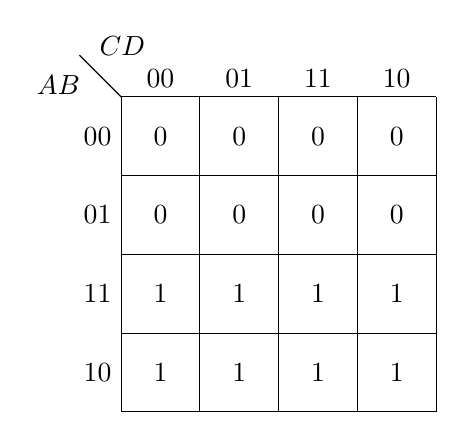
\begin{tikzpicture}
\pgfmathsetmacro{\kxstep}{1}
\pgfmathsetmacro{\kystep}{1}
\pgfmathsetmacro{\kpin}{0.75}
\draw[xstep=\kxstep,ystep=\kystep](0,0) grid (4*\kxstep,-4*\kystep);
\draw(0,0)--++(135:\kpin)node[pos=0.75,above right]{$CD$}node[pos=0.75,below left]{$AB$};
\foreach \kx/\xlb in {0/{00},1/{01},2/{11},3/{10}}{\draw(\kx*\kxstep+\kxstep/2,0)node[above]{$\xlb$};}
\foreach \ky/\ylb in {0/{00},1/{01},2/{11},3/{10}}{\draw(0,-\ky*\kystep-\kystep/2)node[left]{$\ylb$};}
\foreach \kx/\xlb in {0/0,1/0,2/0,3/0}{\draw(\kx*\kxstep+\kxstep/2,-\kystep/2)node[]{$\xlb$};}
\foreach \kx/\xlb in {0/0,1/0,2/0,3/0}{\draw(\kx*\kxstep+\kxstep/2,-1.5*\kystep)node[]{$\xlb$};}
\foreach \kx/\xlb in {0/1,1/1,2/1,3/1}{\draw(\kx*\kxstep+\kxstep/2,-2.5*\kystep)node[]{$\xlb$};}
\foreach \kx/\xlb in {0/1,1/1,2/1,3/1}{\draw(\kx*\kxstep+\kxstep/2,-3.5*\kystep)node[]{$\xlb$};}
\end{tikzpicture}
\end{center}

\انتہا{سوال}
%---------------------
\ابتدا{سوال}
جدول \حوالہ{جدول_کارناف_سوالات_الف}-الف  کے  \عددی{Y_3} کا کارناف نقشہ  بنائیں۔ اس سے سادہ ترین مساوات حاصل کر کے عددی دور تخلیق دیں۔
\begin{table}
\centering
\caption{تفاعلات کے  جدول }
\label{جدول_کارناف_سوالات_الف}
\begin{subtable}{0.45\textwidth}
\caption{}
\centering
\begin{otherlanguage}{english}
\begin{tabular}{CCCC|CCCC}
\toprule
A&B&C&D&Y_3&Y_2&Y_1&Y_0\\
\midrule
0&0&0&0&1&0&1&0\\
0&0&0&1&0&1&0&1\\
0&0&1&0&0&1&1&1\\
0&0&1&1&1&0&0&1\\
0&1&0&0&0&0&1&1\\
0&1&0&1&1&0&0&0\\
0&1&1&0&1&1&1&0\\
0&1&1&1&1&1&1&1\\
1&0&0&0&0&0&0&0\\
1&0&0&1&0&0&0&1\\
1&0&1&0&1&0&1&1\\
1&0&1&1&0&1&0&0\\
1&1&0&0&0&1&1&0\\
1&1&0&1&1&0&1&0\\
1&1&1&0&1&1&0&0\\
1&1&1&1&1&1&0&1\\
\bottomrule
\end{tabular}
\end{otherlanguage}
\end{subtable}\hfill
\begin{subtable}{0.45\textwidth}
\caption{}
\centering
\begin{otherlanguage}{english}
\begin{tabular}{CCCC|CCCC}
\toprule
A&B&C&D&Y_3&Y_2&Y_1&Y_0\\
\midrule
0&0&0&0&1&0&1&0\\
0&0&0&1&0&1&0&1\\
0&0&1&0&0&1&1&1\\
0&0&1&1&1&0&0&1\\
0&1&0&0&0&0&1&1\\
0&1&0&1&1&0&0&0\\
0&1&1&0&1&1&1&0\\
0&1&1&1&1&1&1&1\\
1&0&0&0&0&0&0&0\\
1&0&0&1&0&0&0&1\\
1&0&1&0&x&x&x&x\\
1&0&1&1&x&x&x&x\\
1&1&0&0&x&x&x&x\\
1&1&0&1&x&x&x&x\\
1&1&1&0&x&x&x&x\\
1&1&1&1&x&x&x&x\\
\bottomrule
\end{tabular}
\end{otherlanguage}
\end{subtable}
\end{table}
\انتہا{سوال}
%-----------------------
\ابتدا{سوال}
جدول \حوالہ{جدول_کارناف_سوالات_الف}-الف  کے  \عددی{Y_2}   مخارج کا کارناف نقشہ  بنا کر  سادہ ترین عددی دور تخلیق دیں۔


جواب:\quad

\begin{minipage}{0.45\textwidth}
\centering
\begin{tikzpicture}
\pgfmathsetmacro{\kxstep}{1}
\pgfmathsetmacro{\kystep}{1}
\pgfmathsetmacro{\kpin}{0.75}
\pgfmathsetmacro{\kmv}{0.15}
\pgfmathsetmacro{\kmva}{0.10}
\draw[xstep=\kxstep,ystep=\kystep](0,0) grid (4*\kxstep,-4*\kystep);
\draw(0,0)--++(135:\kpin)node[pos=0.75,above right]{$CD$}node[pos=0.75,below left]{$AB$};
\foreach \kx/\xlb in {0/{00},1/{01},2/{11},3/{10}}{\draw(\kx*\kxstep+\kxstep/2,0)node[above]{$\xlb$};}
\foreach \ky/\ylb in {0/{00},1/{01},2/{11},3/{10}}{\draw(0,-\ky*\kystep-\kystep/2)node[left]{$\ylb$};}
\foreach \kx/\xlb in {0/0,1/1,2/0,3/1}{\draw(\kx*\kxstep+\kxstep/2,-\kystep/2)node[]{$\xlb$};}
\foreach \kx/\xlb in {0/0,1/0,2/1,3/1}{\draw(\kx*\kxstep+\kxstep/2,-1.5*\kystep)node[]{$\xlb$};}
\foreach \kx/\xlb in {0/1,1/0,2/1,3/1}{\draw(\kx*\kxstep+\kxstep/2,-2.5*\kystep)node[]{$\xlb$};}
\foreach \kx/\xlb in {0/0,1/0,2/1,3/0}{\draw(\kx*\kxstep+\kxstep/2,-3.5*\kystep)node[]{$\xlb$};}
\draw[gray,dashed] ($(1*\kxstep,-0*\kystep)+(\kmv,-\kmv)$) rectangle ($(2*\kxstep,-1*\kystep)+(-\kmv,\kmv)$);
\draw[gray,dashed] ($(3*\kxstep,-0*\kystep)+(\kmv,-\kmv)$) rectangle ($(4*\kxstep,-2*\kystep)+(-\kmv,\kmv)$);
\draw[gray,dashed] ($(2*\kxstep,-1*\kystep)+(\kmva,-\kmva)$) rectangle ($(4*\kxstep,-3*\kystep)+(-\kmva,\kmva)$);
\draw[gray,dashed] ($(2*\kxstep,-2*\kystep)+(\kmv,-\kmv)$) rectangle ($(3*\kxstep,-4*\kystep)+(-\kmv,\kmv)$);
\draw[gray,dashed] ($(0*\kxstep,-2*\kystep)+(-\kmv,-\kmv)$) --++(1*\kxstep,-0*\kystep)--++(0,-\kystep+2.5*\kmv)--++(-\kxstep,0);
\draw[gray,dashed] ($(4*\kxstep,-2*\kystep)+(\kmv,-\kmv)$) --++(-1*\kxstep,-0*\kystep)--++(0,-\kystep+2.5*\kmv)--++(\kxstep,0);
\end{tikzpicture}
\end{minipage}\hfill
\begin{minipage}{0.55\textwidth}
\centering
\begin{tikzpicture}
\pgfmathsetmacro{\kxstep}{1}
\pgfmathsetmacro{\kystep}{1}
\pgfmathsetmacro{\kpin}{0.75}
\pgfmathsetmacro{\ksepX}{0.25}
\pgfmathsetmacro{\ksepY}{1}
\pgfmathsetmacro{\kW}{0.3}
\draw(0,0)node[or  port,number inputs=5,anchor=out](u1){};
\draw(u1.out)node[right]{$Y$};
\draw[thin](u1.in 1)--++(0,2*\ksepY)--++(-\ksepX,0)node[and port,anchor=out](u2){};
\draw[thin](u1.in 2)--++(-\ksepX,0)--++(0,\ksepY)node[and port,anchor=out,number inputs=3](u3){};
\draw[thin](u1.in 3)--++(-\ksepX,0)node[and port,anchor=out,number inputs=3](u4){};
\draw[thin](u1.in 4)--++(-\ksepX,0)--++(0,-\ksepY)node[and port,anchor=out,number inputs=3](u5){};
\draw[thin](u1.in 5)--++(0,-2*\ksepY)--++(-\ksepX,0)node[and port,anchor=out,number inputs=4](u6){};
\foreach \n/\lbl in {0/{\overline{D}},1/{D},2/{\overline{C}},3/{C},4/{\overline{B}},5/{B},6/{\overline{A}},7/{A}}\draw[thin](u2.in 1)++(-\ksepX-\n*\kW,\kW)node[above]{$\lbl$}coordinate(w\n)coordinate(kA)--($(kA|-u6.in 4)+(0,-\kW)$);
\draw(u2.in 1)coordinate(kA)--(kA-| w5);
\draw(u2.in 2)coordinate(kA)--(kA-| w3);
\draw(u3.in 1)coordinate(kA)--(kA-| w6);
\draw(u3.in 2)coordinate(kA)--(kA-| w3);
\draw(u3.in 3)coordinate(kA)--(kA-| w0);
\draw(u4.in 1)coordinate(kA)--(kA-| w7);
\draw(u4.in 2)coordinate(kA)--(kA-| w3);
\draw(u4.in 3)coordinate(kA)--(kA-| w1);
\draw(u5.in 1)coordinate(kA)--(kA-| w7);
\draw(u5.in 2)coordinate(kA)--(kA-| w5);
\draw(u5.in 3)coordinate(kA)--(kA-| w0);
\draw(u6.in 1)coordinate(kA)--(kA-| w6);
\draw(u6.in 2)coordinate(kA)--(kA-| w4);
\draw(u6.in 3)coordinate(kA)--(kA-| w2);
\draw(u6.in 4)coordinate(kA)--(kA-| w1);
\end{tikzpicture}
\end{minipage}
\انتہا{سوال}
%-------------------------------
\ابتدا{سوال}
جدول \حوالہ{جدول_کارناف_سوالات_الف}-الف  کے  \عددی{Y_1}   مخارج کا کارناف نقشہ  بنا کر  سادہ ترین عددی دور تخلیق دیں۔
\انتہا{سوال}
%-------------------------
\ابتدا{سوال}
جدول \حوالہ{جدول_کارناف_سوالات_الف}-الف  کے  \عددی{Y_0}   مخارج کا کارناف نقشہ  بنا کر  سادہ ترین عددی دور تخلیق دیں۔

جواب:

\begin{minipage}{0.45\textwidth}
\centering
\begin{tikzpicture}
\pgfmathsetmacro{\kxstep}{1}
\pgfmathsetmacro{\kystep}{1}
\pgfmathsetmacro{\kpin}{0.75}
\pgfmathsetmacro{\kmv}{0.15}
\pgfmathsetmacro{\kmva}{0.10}
\draw[xstep=\kxstep,ystep=\kystep](0,0) grid (4*\kxstep,-4*\kystep);
\draw(0,0)--++(135:\kpin)node[pos=0.75,above right]{$CD$}node[pos=0.75,below left]{$AB$};
\foreach \kx/\xlb in {0/{00},1/{01},2/{11},3/{10}}{\draw(\kx*\kxstep+\kxstep/2,0)node[above]{$\xlb$};}
\foreach \ky/\ylb in {0/{00},1/{01},2/{11},3/{10}}{\draw(0,-\ky*\kystep-\kystep/2)node[left]{$\ylb$};}
\foreach \kx/\xlb in {0/0,1/1,2/1,3/1}{\draw(\kx*\kxstep+\kxstep/2,-\kystep/2)node[]{$\xlb$};}
\foreach \kx/\xlb in {0/1,1/0,2/1,3/0}{\draw(\kx*\kxstep+\kxstep/2,-1.5*\kystep)node[]{$\xlb$};}
\foreach \kx/\xlb in {0/0,1/0,2/1,3/0}{\draw(\kx*\kxstep+\kxstep/2,-2.5*\kystep)node[]{$\xlb$};}
\foreach \kx/\xlb in {0/0,1/1,2/0,3/1}{\draw(\kx*\kxstep+\kxstep/2,-3.5*\kystep)node[]{$\xlb$};}
\draw[gray,dashed] ($(0*\kxstep,-1*\kystep)+(\kmv,-\kmv)$) rectangle ($(1*\kxstep,-2*\kystep)+(-\kmv,\kmv)$);
\draw[gray,dashed] ($(2*\kxstep,-1*\kystep)+(\kmv,-\kmv)$) rectangle ($(3*\kxstep,-3*\kystep)+(-\kmv,\kmv)$);
\draw[gray,dashed] ($(2*\kxstep,-0*\kystep)+(\kmva,-\kmva)$) rectangle ($(4*\kxstep,-1*\kystep)+(-\kmva,\kmva)$);
\draw[gray,dashed] ($(1*\kxstep,-0*\kystep)+(\kmv,\kmv)$) --++(0*\kxstep,-1*\kystep) --++(1*\kxstep-2*\kmv,-0*\kystep+0*\kmv) --++(-0*\kxstep,1*\kystep);
\draw[gray,dashed] ($(1*\kxstep,-4*\kystep)+(\kmv,-\kmv)$) --++(0*\kxstep,1*\kystep)--++(1*\kxstep-2*\kmv,-0*\kystep+0*\kmv)--++(-0*\kxstep,-1*\kystep);
\draw[gray,dashed] ($(3*\kxstep,-0*\kystep)+(\kmv,\kmv)$) --++(0*\kxstep,-1*\kystep+\kmv) --++(1*\kxstep-2.5*\kmv,-0*\kystep+0*\kmv) --++(-0*\kxstep,1*\kystep);
\draw[gray,dashed] ($(3*\kxstep,-4*\kystep)+(\kmv,-\kmv)$) --++(0*\kxstep,1*\kystep)--++(1*\kxstep-2*\kmv,-0*\kystep+0*\kmv)--++(-0*\kxstep,-1*\kystep);
%\draw[gray,dashed] ($(4*\kxstep,-2*\kystep)+(\kmv,-\kmv)$) --++(-1*\kxstep,-0*\kystep)--++(0,-\kystep+2.5*\kmv)--++(\kxstep,0);
\end{tikzpicture}
\end{minipage}\hfill
\begin{minipage}{0.55\textwidth}
\centering
\begin{tikzpicture}
\pgfmathsetmacro{\kxstep}{1}
\pgfmathsetmacro{\kystep}{1}
\pgfmathsetmacro{\kpin}{0.75}
\pgfmathsetmacro{\ksepX}{0.25}
\pgfmathsetmacro{\ksepY}{1}
\pgfmathsetmacro{\kW}{0.3}
\draw(0,0)node[or  port,number inputs=5,anchor=out](u1){};
\draw(u1.out)node[right]{$Y$};
\draw[thin](u1.in 1)--++(0,2*\ksepY)--++(-\ksepX,0)node[and port,anchor=out,number inputs=4](u2){};
\draw[thin](u1.in 2)--++(-\ksepX,0)--++(0,\ksepY)node[and port,anchor=out,number inputs=3](u3){};
\draw[thin](u1.in 3)--++(-\ksepX,0)node[and port,anchor=out,number inputs=3](u4){};
\draw[thin](u1.in 4)--++(-\ksepX,0)--++(0,-\ksepY)node[and port,anchor=out,number inputs=3](u5){};
\draw[thin](u1.in 5)--++(0,-2*\ksepY)--++(-\ksepX,0)node[and port,anchor=out,number inputs=3](u6){};
\foreach \n/\lbl in {0/{\overline{D}},1/{D},2/{\overline{C}},3/{C},4/{\overline{B}},5/{B},6/{\overline{A}},7/{A}}\draw[thin](u2.in 1)++(-\ksepX-\n*\kW,\kW)node[above]{$\lbl$}coordinate(w\n)coordinate(kA)--($(kA|-u6.in 3)+(0,-\kW)$);
\draw(u2.in 1)coordinate(kA)--(kA-| w6);
\draw(u2.in 2)coordinate(kA)--(kA-| w5);
\draw(u2.in 3)coordinate(kA)--(kA-| w2);
\draw(u2.in 4)coordinate(kA)--(kA-| w0);
\draw(u3.in 1)coordinate(kA)--(kA-| w5);
\draw(u3.in 2)coordinate(kA)--(kA-| w3);
\draw(u3.in 3)coordinate(kA)--(kA-| w1);
\draw(u4.in 1)coordinate(kA)--(kA-| w6);
\draw(u4.in 2)coordinate(kA)--(kA-| w4);
\draw(u4.in 3)coordinate(kA)--(kA-| w3);
\draw(u5.in 1)coordinate(kA)--(kA-| w4);
\draw(u5.in 2)coordinate(kA)--(kA-| w2);
\draw(u5.in 3)coordinate(kA)--(kA-| w1);
\draw(u6.in 1)coordinate(kA)--(kA-| w4);
\draw(u6.in 2)coordinate(kA)--(kA-| w3);
\draw(u6.in 3)coordinate(kA)--(kA-| w0);
\end{tikzpicture}
\end{minipage}
\انتہا{سوال}
%-------------------------
\ابتدا{سوال}
جدول \حوالہ{جدول_کارناف_سوالات_الف}-ب  کے  \عددی{Y_3}   مخارج کا کارناف نقشہ  بنا کر  سادہ ترین عددی دور تخلیق دیں۔
\انتہا{سوال}
%-------------------------
\ابتدا{سوال}
جدول \حوالہ{جدول_کارناف_سوالات_الف}-ب کے  \عددی{Y_2}   مخارج کا کارناف نقشہ  بنا کر  سادہ ترین عددی دور تخلیق دیں۔

جواب:


\begin{minipage}{0.45\textwidth}
\centering
\begin{tikzpicture}
\pgfmathsetmacro{\kxstep}{1}
\pgfmathsetmacro{\kystep}{1}
\pgfmathsetmacro{\kpin}{0.75}
\pgfmathsetmacro{\kmv}{0.15}
\pgfmathsetmacro{\kmva}{0.10}
\draw[xstep=\kxstep,ystep=\kystep](0,0) grid (4*\kxstep,-4*\kystep);
\draw(0,0)--++(135:\kpin)node[pos=0.75,above right]{$CD$}node[pos=0.75,below left]{$AB$};
\foreach \kx/\xlb in {0/{00},1/{01},2/{11},3/{10}}{\draw(\kx*\kxstep+\kxstep/2,0)node[above]{$\xlb$};}
\foreach \ky/\ylb in {0/{00},1/{01},2/{11},3/{10}}{\draw(0,-\ky*\kystep-\kystep/2)node[left]{$\ylb$};}
\foreach \kx/\xlb in {0/0,1/1,2/0,3/1}{\draw(\kx*\kxstep+\kxstep/2,-\kystep/2)node[]{$\xlb$};}
\foreach \kx/\xlb in {0/0,1/0,2/1,3/1}{\draw(\kx*\kxstep+\kxstep/2,-1.5*\kystep)node[]{$\xlb$};}
\foreach \kx/\xlb in {0/x,1/x,2/x,3/x}{\draw(\kx*\kxstep+\kxstep/2,-2.5*\kystep)node[]{$\xlb$};}
\foreach \kx/\xlb in {0/0,1/0,2/x,3/x}{\draw(\kx*\kxstep+\kxstep/2,-3.5*\kystep)node[]{$\xlb$};}
\draw[gray,dashed] ($(1*\kxstep,-0*\kystep)+(\kmv,-\kmv)$) rectangle ($(2*\kxstep,-1*\kystep)+(-\kmv,\kmv)$);
\draw[gray,dashed] ($(2*\kxstep,-1*\kystep)+(\kmv,-\kmv)$) rectangle ($(4*\kxstep,-3*\kystep)+(-1.5*\kmv,\kmv)$);
\draw[gray,dashed] ($(3*\kxstep,-0*\kystep)+(\kmva,-\kmva)$) rectangle ($(4*\kxstep,-4*\kystep)+(-\kmva,\kmva)$);
%\draw[gray,dashed] ($(4*\kxstep,-2*\kystep)+(\kmv,-\kmv)$) --++(-1*\kxstep,-0*\kystep)--++(0,-\kystep+2.5*\kmv)--++(\kxstep,0);
\end{tikzpicture}
\end{minipage}\hfill
\begin{minipage}{0.55\textwidth}
\centering
\begin{tikzpicture}
\pgfmathsetmacro{\kxstep}{1}
\pgfmathsetmacro{\kystep}{1}
\pgfmathsetmacro{\kpin}{0.75}
\pgfmathsetmacro{\ksepX}{0.25}
\pgfmathsetmacro{\ksepY}{1}
\pgfmathsetmacro{\kW}{0.3}
\draw(0,0)node[or  port,number inputs=3,anchor=out](u1){};
\draw(u1.out)node[right]{$Y$};
\draw[thin](u1.in 1)--++(0,1*\ksepY)--++(-\ksepX,0)node[and port,anchor=out,number inputs=4](u2){};
\draw[thin](u1.in 2)--++(-\ksepX,0)node[and port,anchor=out,number inputs=2](u3){};
\draw[thin](u1.in 3)--++(0,-1*\ksepY)--++(-\ksepX,0)node[and port,anchor=out,number inputs=2](u4){};
\foreach \n/\lbl in {0/{\overline{D}},1/{D},2/{\overline{C}},3/{C},4/{\overline{B}},5/{B},6/{\overline{A}},7/{A}}\draw[thin](u2.in 1)++(-\ksepX-\n*\kW,\kW)node[above]{$\lbl$}coordinate(w\n)coordinate(kA)--($(kA|-u4.in 2)+(0,-\kW)$);
\draw(u2.in 1)coordinate(kA)--(kA-| w6);
\draw(u2.in 2)coordinate(kA)--(kA-| w4);
\draw(u2.in 3)coordinate(kA)--(kA-| w2);
\draw(u2.in 4)coordinate(kA)--(kA-| w1);
\draw(u3.in 1)coordinate(kA)--(kA-| w5);
\draw(u3.in 2)coordinate(kA)--(kA-| w3);
\draw(u4.in 1)coordinate(kA)--(kA-| w3);
\draw(u4.in 2)coordinate(kA)--(kA-| w0);
\end{tikzpicture}
\end{minipage}
\انتہا{سوال}
%-------------------------
\ابتدا{سوال}
جدول \حوالہ{جدول_کارناف_سوالات_الف}-ب کے  \عددی{Y_1}   مخارج کا کارناف نقشہ  بنا کر  سادہ ترین عددی دور تخلیق دیں۔
\انتہا{سوال}
%-------------------------
\ابتدا{سوال}
جدول \حوالہ{جدول_کارناف_سوالات_الف}-ب کے  \عددی{Y_0}   مخارج کا کارناف نقشہ  بنا کر  سادہ ترین عددی دور تخلیق دیں۔

جواب:

\begin{minipage}{0.45\textwidth}
\centering
\begin{tikzpicture}
\pgfmathsetmacro{\kxstep}{1}
\pgfmathsetmacro{\kystep}{1}
\pgfmathsetmacro{\kpin}{0.75}
\pgfmathsetmacro{\kmv}{0.15}
\pgfmathsetmacro{\kmva}{0.10}
\draw[xstep=\kxstep,ystep=\kystep](0,0) grid (4*\kxstep,-4*\kystep);
\draw(0,0)--++(135:\kpin)node[pos=0.75,above right]{$CD$}node[pos=0.75,below left]{$AB$};
\foreach \kx/\xlb in {0/{00},1/{01},2/{11},3/{10}}{\draw(\kx*\kxstep+\kxstep/2,0)node[above]{$\xlb$};}
\foreach \ky/\ylb in {0/{00},1/{01},2/{11},3/{10}}{\draw(0,-\ky*\kystep-\kystep/2)node[left]{$\ylb$};}
\foreach \kx/\xlb in {0/0,1/1,2/1,3/1}{\draw(\kx*\kxstep+\kxstep/2,-\kystep/2)node[]{$\xlb$};}
\foreach \kx/\xlb in {0/1,1/0,2/1,3/0}{\draw(\kx*\kxstep+\kxstep/2,-1.5*\kystep)node[]{$\xlb$};}
\foreach \kx/\xlb in {0/x,1/x,2/x,3/x}{\draw(\kx*\kxstep+\kxstep/2,-2.5*\kystep)node[]{$\xlb$};}
\foreach \kx/\xlb in {0/0,1/1,2/x,3/x}{\draw(\kx*\kxstep+\kxstep/2,-3.5*\kystep)node[]{$\xlb$};}
\draw[gray,dashed] ($(0*\kxstep,-1*\kystep)+(\kmv,-\kmv)$) rectangle ($(1*\kxstep,-3*\kystep)+(-\kmv,\kmv)$);
\draw[gray,dashed] ($(2*\kxstep,-0*\kystep)+(\kmv,-\kmv)$) rectangle ($(3*\kxstep,-4*\kystep)+(-\kmv,\kmv)$);
\draw[gray,dashed] ($(1*\kxstep,-0*\kystep)+(\kmv,\kmv)$) --++(0*\kxstep,-1*\kystep) --++(2*\kxstep-2.5*\kmv,-0*\kystep+0*\kmv) --++(-0*\kxstep,1*\kystep);
\draw[gray,dashed] ($(1*\kxstep,-4*\kystep)+(\kmv,-1.5*\kmv)$) --++(0*\kxstep,1*\kystep) --++(2*\kxstep-2.5*\kmv,-0*\kystep+0*\kmv) --++(-0*\kxstep,-1*\kystep);
\draw[gray,dashed] ($(2*\kxstep,-0*\kystep)+(1.5*\kmv,1.5*\kmv)$) --++(0*\kxstep,-1*\kystep-2.5*\kmv) --++(2*\kxstep-2.5*\kmv,-0*\kystep+0*\kmv) --++(-0*\kxstep,1*\kystep+2.5*\kmv);
\draw[gray,dashed] ($(2*\kxstep,-4*\kystep)+(1.5*\kmv,-1.5*\kmv)$) --++(0*\kxstep,1*\kystep+1*\kmv) --++(2*\kxstep-2.5*\kmv,-0*\kystep+0*\kmv) --++(-0*\kxstep,-1*\kystep-1*\kmv);
\end{tikzpicture}
\end{minipage}\hfill
\begin{minipage}{0.55\textwidth}
\centering
\begin{tikzpicture}
\pgfmathsetmacro{\kxstep}{1}
\pgfmathsetmacro{\kystep}{1}
\pgfmathsetmacro{\kpin}{0.75}
\pgfmathsetmacro{\ksepX}{0.25}
\pgfmathsetmacro{\ksepY}{1}
\pgfmathsetmacro{\kW}{0.3}
\draw(0,0)node[or  port,number inputs=4,anchor=out](u1){};
\draw(u1.out)node[right]{$Y$};
\draw[thin](u1.in 1)--++(0,1.5*\ksepY)--++(-\ksepX,0)node[and port,anchor=out,number inputs=3](u2){};
\draw[thin](u1.in 2)--++(-\ksepX,0)--++(0,0.5*\ksepY)node[and port,anchor=out,number inputs=2](u3){};
\draw[thin](u1.in 3)--++(-\ksepX,0)--++(0,-0.5*\ksepY)node[and port,anchor=out,number inputs=2](u4){};
\draw[thin](u1.in 4)--++(0,-1.5*\ksepY)--++(-\ksepX,0)node[and port,anchor=out,number inputs=2](u5){};
\foreach \n/\lbl in {0/{\overline{D}},1/{D},2/{\overline{C}},3/{C},4/{\overline{B}},5/{B},6/{\overline{A}},7/{A}}\draw[thin](u2.in 1)++(-\ksepX-\n*\kW,\kW)node[above]{$\lbl$}coordinate(w\n)coordinate(kA)--($(kA|-u5.in 2)+(0,-\kW)$);
\draw(u2.in 1)coordinate(kA)--(kA-| w5);
\draw(u2.in 2)coordinate(kA)--(kA-| w2);
\draw(u2.in 3)coordinate(kA)--(kA-| w0);
\draw(u3.in 1)coordinate(kA)--(kA-| w4);
\draw(u3.in 2)coordinate(kA)--(kA-| w3);
\draw(u4.in 1)coordinate(kA)--(kA-| w4);
\draw(u4.in 2)coordinate(kA)--(kA-| w1);
\draw(u5.in 1)coordinate(kA)--(kA-| w3);
\draw(u5.in 2)coordinate(kA)--(kA-| w1);
\end{tikzpicture}
\end{minipage}
\انتہا{سوال}
%-------------------------
